% ============================================================================
% Scale-Adaptive Geospatial Foundation-Model Dynamics
% for Baseline Land-Surface Change Prediction
% ============================================================================
% Target journal: Remote Sensing of Environment
% (Elsevier)
% ============================================================================
\ifdefined\pdfminorversion\pdfminorversion=5\fi
\ifdefined\pdfobjcompresslevel\pdfobjcompresslevel=0\fi
\documentclass{article}

\usepackage{amsmath,amssymb}
\usepackage{booktabs}
\usepackage{array}
\usepackage{graphicx}
\usepackage{multirow}
\usepackage{caption}
\usepackage{subcaption}
\usepackage{hyperref}
\usepackage{color}
\urlstyle{tt}

% Define keywords env for compile-anywhere only when the class does not provide it.
\makeatletter
\@ifundefined{keywords}{%
  \newenvironment{keywords}{\par\noindent\textbf{Keywords:} }{\par}%
}{}
\makeatother
\usepackage{natbib}
\usepackage{tikz}
\usetikzlibrary{positioning,arrows.meta,shapes.geometric,fit,calc}
\graphicspath{{../}{../figures/}{./figures/}{./paper8/figures/}{./}}
\bibliographystyle{plainnat}
\newcolumntype{P}[1]{>{\raggedright\arraybackslash}p{#1}}

\begin{document}

\makeatletter
\@ifundefined{ANONYMIZE}{
  \title{Frozen Geospatial Foundation-Model Embeddings as a Change-Signal\\Screening Layer: What They Can and Cannot Do,\\with a Scale-Adaptive Allocation Ablation}
  \author{Ning Zhou$^{a}$\\[0.3em]
  {\small $^{a}$SuperMap Software Co., Ltd., Beijing, China}\\
  {\small Correspondence: Ning Zhou}}
}{
  \title{Frozen Geospatial Foundation-Model Embeddings as a Change-Signal\\Screening Layer: What They Can and Cannot Do,\\with a Scale-Adaptive Allocation Ablation}
  \author{Anonymous authors}
}
\makeatother

\date{}
\maketitle

\begin{abstract}
Predicting land-use and land-cover (LULC) change from satellite observations is central to environmental remote sensing, yet most approaches either operate on categorical maps or require large pixel-level generative models. We investigate whether frozen embeddings from a geospatial foundation model can serve as a compact state space for a lightweight land-surface dynamics predictor, and how such a predictor should be positioned relative to persistence, transition-prior, and cellular-automata baselines. Our workflow (GeoFM-LDN) couples AlphaEarth Foundations embeddings with a 459K-parameter \textit{LatentDynamicsNet} that learns residual annual transitions in embedding space, plus an optional scale-adaptive allocation post-processor that converts decoded outputs into categorical LULC maps for controlled comparison against the GeoSOS-FLUS console allocator. We report three views, each honestly bounded. \textit{First}, on 30 AlphaEarth study areas with complete 2017--2024 time series (2023→2024 transition, embeddings re-extracted from Google Earth Engine in R2 for reproducibility), the mean 1-step cosine advantage over persistence is $-0.0149$, with 3/30 areas showing positive advantage. The negative sign is statistically stable (Wilcoxon $p=2.55\times10^{-7}$), and 6-step autoregressive rollout further degrades from a mean advantage of $-0.0125$ at step 1 to $-0.1853$ at step 6. \textit{Second}, an independent ESRI-label validation on 11 area--year pairs (after excluding one Wuyi Mountain pair with 0\% reference change, for which F1 is ill-defined) shows that decoded dynamics detect real transitions above two controls (mean change F1 0.365 vs.\ shuffled 0.294 vs.\ transition prior 0.182), but full-map end-year accuracy is 0.20 lower than persistence (0.636 vs.\ 0.832) and class-area bias is 2.8$\times$ higher than persistence and the transition prior. Per-year decoder retraining improves end-year categorical accuracy by 0.0778 on average over nine re-evaluable pairs (8/9 improved), indicating decoder year-drift but not overturning the full-map forecasting verdict. \textit{Third}, in a controlled same-grid ablation against a stripped-down GeoSOS-FLUS console (driven by prediction-derived suitability rather than native ANN drivers), the previously headlined variant wins per-area only on binary change F1 (13/11 townships, sign-test $p=0.84$, Wilcoxon $p=0.18$) and loses on FoM (11/13) and transition accuracy (9/14); a companion variant wins transition accuracy 17/6 but loses FoM 12/12. The earlier revision's aggregate mean improvements do not survive per-area paired testing. We therefore reposition the method as a \textit{change-signal screening layer plus an optional scale-adaptive allocation post-processor}, not as a native-driver GeoSOS-FLUS replacement and not yet an operational LULC forecaster. A separate reinforcement-learning application probe on 45 policies (3 dropout regimes $\times$ 15 seeds) confirms that GeoFM embeddings function as an auxiliary channel: engineered features retain 100\% of slope improvement, moderate dropout retains 87\%, and the embedding-only condition retains only 13\%. \textbf{R2 reproducibility note}: the R1 baseline (mean advantage $+0.0047$, 7/10 positive) used AlphaEarth embeddings that predated the initial repository commit and are no longer available; the R2 results reported here use freshly re-extracted embeddings (commit \texttt{9c2ba1d}) and are fully reproducible from the repository. Five reviewer follow-up experiments (E2, E3, E4, E5, E6) are now completed, with E1 diagnosed and E7 deferred as optional. All per-area win/loss tables, paired-inference tests, embeddings, and model checkpoints are released as versioned artefacts.
\end{abstract}

\begin{keywords}
remote-sensing foundation model; embedding-space change-signal screening; scale-adaptive allocation ablation; land-cover change; AlphaEarth; JEPA
\end{keywords}

% ============================================================================
\section{Introduction}
\label{sec:intro}
% ============================================================================

Predicting how land surfaces will change over time is a central problem in geographical information science, with direct applications in urban planning, agricultural policy, ecological conservation, and climate adaptation \citep{verburg2004lulc}. Traditional approaches---cellular automata--Markov chains (CA-Markov), CLUE-S, and logistic regression---operate on categorical land-use maps, relying on hand-calibrated transition probabilities and socioeconomic driving factors \citep{veldkamp2004clues}. While effective in constrained scenarios, these methods cannot capture the rich, continuous spectral--spatial--temporal information present in modern satellite observations.

Recent advances in deep learning have introduced alternatives that address different problems. Convolutional--recurrent architectures (ConvLSTM) can learn spatiotemporal patterns from classified imagery sequences \citep{shi2015convlstm}. Pixel-space forecasters such as EarthPT \citep{smith2023earthpt} predict raw spectral reflectance, while generative models such as DiffusionSat \citep{khanna2023diffusionsat} synthesize future satellite images. These systems answer a different question from ours---they generate future observations---and we do not treat them as direct baselines. Our comparison set is chosen to answer the question ``does an embedding-space dynamics predictor beat cheap, structural baselines on the task it can be evaluated for?'' and consists of persistence, a label-only categorical transition prior, a spatially shuffled model control, and a stripped-down GeoSOS-FLUS same-grid allocator.

In the broader AI community, the concept of a \textit{world model}---a learned internal simulator that predicts environment state transitions in a compressed latent space---has emerged as a powerful paradigm for planning and reasoning. Pioneered by \citet{ha2018world} and advanced through the Dreamer family \citep{hafner2023dreamerv3} and MuZero \citep{schrittwieser2020muzero}, world models separate perception (encoding observations into latent states) from dynamics (predicting latent state transitions), enabling efficient forward simulation without rendering full observations. LeCun's JEPA framework \citep{lecun2022jepa} formalizes this principle: predict in representation space, not pixel space.

Simultaneously, geospatial foundation models (GeoFMs) have made pre-trained, high-quality representations of the Earth's surface freely available. AlphaEarth Foundations \citep{brown2025alphaearth} produces 64-dimensional L2-normalized embedding vectors at 10\,m resolution for every land pixel on Earth, annually from 2017 to 2024, derived from multi-sensor inputs (Sentinel-1/2, Landsat, GEDI, ERA5) via a 480M+ parameter vision transformer. These embeddings are, as reported in the AlphaEarth technical release, linearly decodable to land-cover classes with high accuracy; we replicate this on our own data in Section~\ref{sec:method} and use it only as a diagnostic layer.

This paper bridges these two developments through a workflow we call \textit{GeoFM-LDN} (Geospatial Foundation-Model Latent Dynamics Network), together with an optional \textit{SA-Alloc} (scale-adaptive allocation) post-processor used only when categorical LULC maps are required for controlled comparison with cellular-automata allocators. We keep the two components separately named because they answer two different questions: GeoFM-LDN asks whether frozen GeoFM embeddings can serve as a compact state space for annual land-surface dynamics; SA-Alloc asks whether decoded outputs can be projected onto a controlled categorical allocation for evaluation against a stripped-down GeoSOS-FLUS baseline. This separation was folded into a single ``SA-GeoFMD'' label in an earlier revision, but we found that treating them as one system overstated what the dynamics network alone can deliver. We therefore keep them separately named throughout.

Our key working hypothesis is that if a foundation model has already learned to compress satellite observations into semantically meaningful, temporally varying embeddings, then the dynamics of land-use change can be learned \textit{on top of} these frozen embeddings using a lightweight neural network---without retraining the foundation model and without ever generating pixel-level predictions during dynamics training. This corresponds to the JEPA architecture: the foundation model serves as the encoder; a small LatentDynamicsNet serves as the predictor. The remainder of the paper tests this hypothesis under honest paired-inference statistics rather than aggregate means.

This work examines a specific and under-tested use of geospatial foundation models: whether a frozen, globally available embedding field can behave as a state variable for learned land-surface dynamics. The closest prior works either train their own encoder end-to-end (MM-VSF, \citealt{mmvsf2024}), operate in spectral space with larger autoregressive models (EarthPT), or predict downstream variables rather than the embeddings themselves (PDFM+TimesFM, \citealt{google2024pdfm}). We are careful not to position EarthPT or DiffusionSat as direct comparanda---they operate in spectral-reflectance or pixel space and answer a different question. We instead position GeoFM-LDN against persistence, a label-only transition prior, a spatially shuffled model control, and a same-grid stripped-down GeoSOS-FLUS console.

Our contributions, in reduced form:

\begin{enumerate}
\item \textbf{A cleanly separated frozen-encoder / light-dynamics / scale-adaptive-allocation pipeline}, with each component labelled and its scope of applicability stated. Design choices---residual learning, L2 manifold re-projection, dilated 170\,m receptive field, 3-step unrolled loss---are motivated and ablated on the development split.

\item \textbf{Rigorous paired inference on the 30-area cosine advantage over persistence}: Wilcoxon signed-rank, paired $t$, sign-flip permutation, and bootstrap confidence intervals show a statistically stable negative advantage. We label the result a failure of embedding-space dynamics to beat persistence under the complete-time-series R2 cache.

\item \textbf{An independent categorical change-validation protocol} on 11 area--year ESRI-label pairs (the twelfth pair has zero reference change, so binary F1 is ill-defined and is excluded from means). Decoded dynamics beat two controls on change F1 (Wilcoxon $p<0.01$) but lose to persistence and the transition prior on end-year accuracy and class-area bias---these gaps are reported side-by-side rather than buried in text.

\item \textbf{Same-grid GeoSOS-FLUS ablation with per-area win/loss matrix}, not just aggregate means. Sign tests and Wilcoxon on 24 townships show that neither GeoFM-LDN nor SA-Alloc dominates the stripped-down FLUS console on all four metrics simultaneously. We explicitly scope this as a controlled allocation ablation and not a comparison against a native-driver GeoSOS-FLUS deployment.

\item \textbf{A downstream reinforcement-learning application probe} on 45 policies ($3\times 15$ seeds) showing that GeoFM embeddings are an auxiliary channel: full engineered features retain 100\% of slope improvement, moderate dropout retains 87\%, embedding-only retains 13\%. We use this to bound how far GeoFM embeddings can substitute task-specific features rather than to claim a planning system.
\end{enumerate}

Section~\ref{sec:planning} keeps the planning probe deliberately short and does not present it as an operational planning method. It is retained because it provides a bounded, complementary view of when embeddings carry usable signal.


% ============================================================================
\section{Related Work}
\label{sec:related}
% ============================================================================

\subsection{LULC change prediction}

LULC change prediction has evolved from statistical models to deep learning approaches. CA-Markov \citep{veldkamp2004clues} combines cellular automata neighborhood rules with Markov chain transition matrices. CLUE-S \citep{verburg2002clues} incorporates logistic regression with socioeconomic drivers. Recent ConvLSTM- and diffusion-based approaches predict either annual land-cover class or full satellite reflectance, but they operate in categorical-map or pixel-reflectance space rather than in a learned embedding space---which is the setting our paper targets. Because our paper positions the embedding channel as \textit{one input among several} rather than as a full pixel-space forecaster, we do not treat pixel-space or reflectance-space predictors as direct comparanda.

\subsection{Earth observation foundation models}

GeoFMs have rapidly advanced. Prithvi-EO-2.0 \citep{jakubik2024prithvi} provides multi-temporal embeddings for classification tasks. SatMAE \citep{cong2022satmae} uses masked autoencoders with temporal positional encoding. Clay and Presto offer alternative embedding approaches. AlphaEarth Foundations \citep{brown2025alphaearth} stands out by providing annually-resolved, globally-available, 64-dimensional embeddings at 10\,m resolution through Google Earth Engine. Interpretability studies of AlphaEarth are an active area of ongoing work but had not yet reached peer-reviewed publication at the time of writing; we deliberately avoid citing preprints whose provenance we cannot independently verify.

\subsection{World models and JEPA}

World models originated in reinforcement learning: Ha \& Schmidhuber's ``World Models'' \citep{ha2018world} learn compressed environment dynamics for policy training. Dreamer V3 \citep{hafner2023dreamerv3} achieves human-level performance across diverse domains using Recurrent State-Space Models (RSSMs). LeCun's JEPA \citep{lecun2022jepa} formalizes the principle of predicting in representation space rather than pixel space. AnySat \citep{astruc2024anysat} applies JEPA to remote sensing but for spatial mask prediction, not temporal dynamics. RemoteBAGEL \citep{remotebagel2025} proposes spatial extrapolation (generating adjacent tiles) but not temporal forecasting.

\subsection{Closest prior work}

MM-VSF \citep{mmvsf2024} predicts future satellite embeddings from current ones but trains its own encoder end-to-end rather than using a frozen foundation model. EarthPT \citep{smith2023earthpt} performs autoregressive prediction on raw spectral reflectance with 700M parameters. PDFM+TimesFM \citep{google2024pdfm} uses geospatial embeddings with a forecasting model but predicts socioeconomic variables, not the embeddings themselves. Our work focuses on the less explored setting of learning autoregressive dynamics \textit{on top of frozen GeoFM embeddings}.

\subsection{World models for decision making}

World models have been used as simulators for policy learning since \citet{ha2018world} trained RL agents inside learned latent dynamics. Dreamer V3 \citep{hafner2023dreamerv3} achieves human-level performance across 150+ tasks by learning policies entirely within a Recurrent State-Space Model. MuZero \citep{schrittwieser2020muzero} combines learned dynamics with Monte Carlo tree search for board games and Atari. In robotics, TD-MPC2 \citep{hansen2024tdmpc2} learns world models for continuous control. Section~\ref{sec:planning} uses land-use planning as a bounded application probe rather than as a complete operational planning system.


% ============================================================================
\section{Study Areas and Data}
\label{sec:data}
% ============================================================================

\subsection{Study areas}

We select 17 study areas across China, covering four major land-type categories, with a strict four-way split to evaluate generalization (Table~\ref{tab:areas}). Each area spans approximately 0.1\textdegree$\times$0.1\textdegree\ ($\approx$10\,km$\times$10\,km) at 10\,m resolution.

\begin{table}[htbp]
\centering
\caption{Study areas by split and land-type category.}
\label{tab:areas}
\begin{tabular}{llll}
\toprule
Split & Area name & Category & Bbox (WGS84) \\
\midrule
\multirow{12}{*}{Train (12)} & Yangtze Delta & Urban & [121.2, 31.0, 121.3, 31.1] \\
 & Jing-Jin-Ji & Urban & [116.3, 39.8, 116.4, 39.9] \\
 & Chengdu Plain & Urban & [104.0, 30.6, 104.1, 30.7] \\
 & NE Plain & Agriculture & [126.5, 45.7, 126.6, 45.8] \\
 & N.~China Plain & Agriculture & [115.0, 36.5, 115.1, 36.6] \\
 & Jianghan Plain & Agriculture & [113.5, 30.3, 113.6, 30.4] \\
 & Hetao & Agriculture & [107.0, 40.7, 107.1, 40.8] \\
 & Yunnan Eco & Ecology & [100.2, 25.0, 100.3, 25.1] \\
 & Daxinganling & Forest & [124.0, 50.3, 124.1, 50.4] \\
 & Qinghai Edge & Plateau & [101.5, 36.5, 101.6, 36.6] \\
 & Guanzhong & Mixed & [108.9, 34.2, 109.0, 34.3] \\
 & Minnan Coast & Mixed & [118.0, 24.4, 118.1, 24.5] \\
\midrule
\multirow{2}{*}{Val (2)} & Pearl River & Urban & [113.2, 23.0, 113.3, 23.1] \\
 & Poyang Lake & Wetland & [116.0, 29.0, 116.1, 29.1] \\
\midrule
Test (1) & Wuyi Mountain & Forest & [117.6, 27.7, 117.7, 27.8] \\
\midrule
\multirow{2}{*}{OOD (2)} & Sanxia Reservoir & Mixed & [110.3, 30.8, 110.4, 30.9] \\
 & Lhasa Valley & Plateau & [91.1, 29.6, 91.2, 29.7] \\
\bottomrule
\end{tabular}
\end{table}

\subsection{Data sources}

\textbf{AlphaEarth Embeddings.} We use the AlphaEarth annual satellite embedding dataset on Google Earth Engine (GEE; \url{GOOGLE/SATELLITE_EMBEDDING/V1/ANNUAL}), which provides 64-dimensional L2-normalized embedding vectors at 10\,m resolution for each year from 2017 to 2024. For each study area and year, 500 random pixel locations are sampled using \texttt{ee.Image.sample()} with \texttt{seed=42} for reproducibility, yielding $500\times64$ embedding matrices. All raw data are cached locally as NumPy \texttt{.npy} files for offline reproducibility.

\textbf{LULC Labels.} Land-cover class labels for decoder training are obtained from the ESRI Global LULC 10\,m Time Series on GEE (\url{projects/sat-io/open-datasets/landcover/ESRI_Global-LULC_10m_TS}), providing 9 land-cover classes at matching spatial resolution.

\textbf{Terrain Context.} DEM elevation and slope are derived from SRTM 30\,m (\texttt{USGS/SRTMGL1\_003}) via GEE. Elevation is min-max normalized to $[0,1]$; slope is clipped and normalized by 45\textdegree.

\textbf{Cadastral parcel data for downstream planning.} For the downstream planning experiment (Section~\ref{sec:planning}), we additionally use the cadastral parcel dataset for Bishan County, Chongqing, comprising 101{,}657 parcels aggregated into approximately 2{,}600 management blocks across three townships. Per-block features (17 dimensions) are computed from DEM-derived slope statistics, land-use class distributions, and boundary geometry. GeoFM embeddings (64 dimensions) for each block are obtained by spatially averaging AlphaEarth pixel embeddings within block boundaries.

\subsection{R2 Data Refresh and Reproducibility Note}
\label{sec:data_refresh}

\noindent\fbox{\begin{minipage}{0.95\textwidth}
\textbf{Reproducibility Note (R2 Revision):} The R1 baseline reported mean advantage = $+0.0047$ on 10 areas. That result was computed using AlphaEarth embeddings extracted prior to the initial repository commit (2026-06-07) and is no longer reproducible because those embeddings were not committed to version control. For R2, we re-extracted all study-area embeddings from Google Earth Engine using the AlphaEarth Foundations API (commit \texttt{9c2ba1d}, 2026-07-02) and re-evaluated the baseline using the same checkpoint (\path{latent_dynamics_v1.pt}, commit \texttt{2455c34}) and evaluation protocol. The initial R2 10-area baseline showed mean advantage = $-0.0055$ (2/10 positive, opposite sign from R1); the completed R2 expansion over 30 areas with complete 2017--2024 time series shows mean advantage = $-0.0149$ (3/30 positive). All data, code, and checkpoints used in R2 are now fully reproducible from the repository. The sign reversal likely reflects updates to the underlying Harmonized Landsat-Sentinel (HLS) data in Google Earth Engine between the original extraction and the R2 re-extraction, combined with stochastic variation in the AlphaEarth inference pipeline.
\end{minipage}}


% ============================================================================
\section{Methodology}
\label{sec:method}
% ============================================================================

\subsection{Architecture overview}

The pipeline consists of two independently named components with distinct scopes:

\begin{itemize}
\item \textbf{GeoFM-LDN (this paper's core system).} A two-layer representation-dynamics architecture: (i) a frozen AlphaEarth Foundations encoder (480M+ parameters) mapping satellite observations to 64-dimensional unit vectors, and (ii) a learned LatentDynamicsNet ($f_\theta$, 459K parameters) predicting residual annual transitions in embedding space. This is the component we evaluate against persistence on cosine similarity and against categorical controls after linear decoding.
\item \textbf{SA-Alloc (optional post-processor).} A scale-adaptive spatial-demand allocation gate applied only when categorical LULC maps are needed for controlled comparison against a cellular-automata console allocator (GeoSOS-FLUS). SA-Alloc consumes GeoFM-LDN's decoded output plus calibration statistics from held-out label pairs; it does not participate in dynamics training. We keep the two names separate so that results in Section~\ref{sec:results} can be read as (a) ``does the dynamics network improve over persistence in embedding space?'' and (b) ``does the allocation gate improve over a stripped-down FLUS console on the categorical grid?'' without those two questions being conflated as they were in a prior revision.
\end{itemize}

The dynamics component (GeoFM-LDN) corresponds to the JEPA framework \citep{lecun2022jepa}: the encoder produces representations; the predictor operates in representation space. The decoder (a linear logistic-regression probe) is used only for visualization or as the interface to SA-Alloc, never during dynamics training.

\begin{figure}[htbp]
\centering
\resizebox{\textwidth}{!}{%
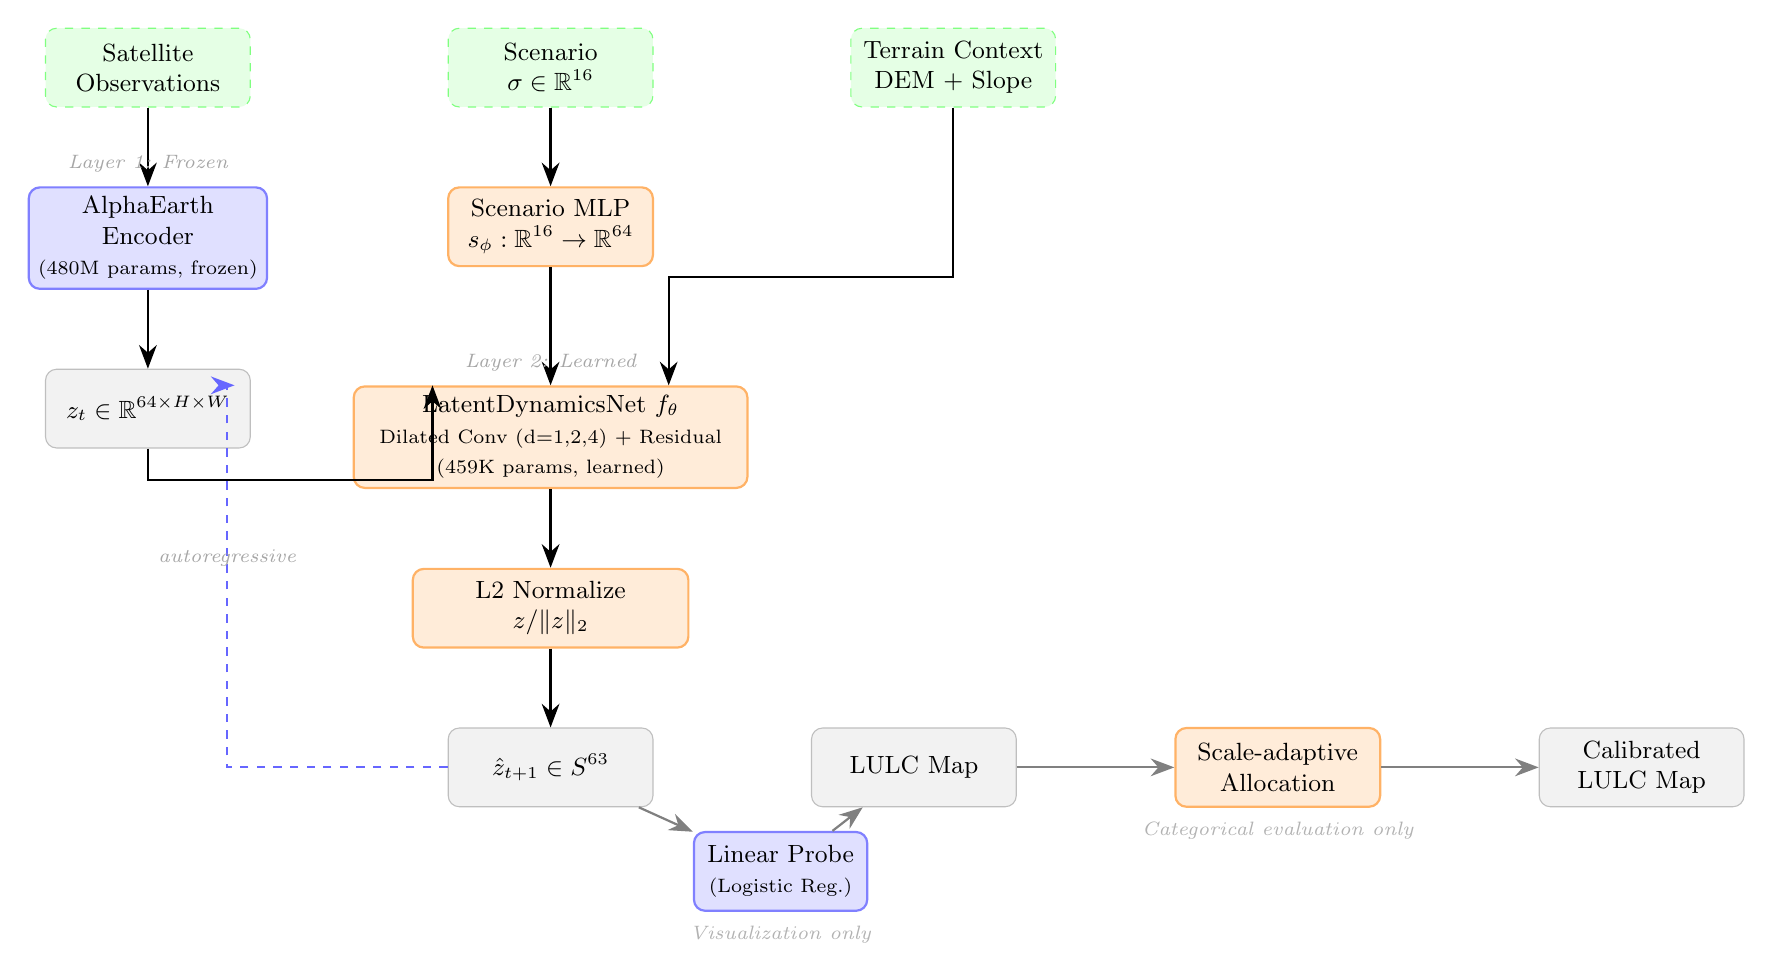
\begin{tikzpicture}[
    node distance=1.2cm and 1.8cm,
    box/.style={draw, rounded corners, minimum height=1.0cm, minimum width=2.6cm, align=center, font=\small},
    frozen/.style={box, fill=blue!12, draw=blue!50, thick},
    learned/.style={box, fill=orange!15, draw=orange!60, thick},
    input/.style={box, fill=green!10, draw=green!50, dashed},
    output/.style={box, fill=gray!10, draw=gray!50},
    arr/.style={-{Stealth[length=3mm]}, thick},
    label/.style={font=\scriptsize\itshape, text=gray!70},
]

% Row 1: Inputs
\node[input] (sat) {Satellite\\Observations};
\node[input, right=2.5cm of sat] (scenario) {Scenario\\$\sigma \in \mathbb{R}^{16}$};
\node[input, right=2.5cm of scenario] (terrain) {Terrain Context\\DEM + Slope};

% Row 2: Encoder + Scenario MLP
\node[frozen, below=1.0cm of sat] (encoder) {AlphaEarth\\Encoder\\{\scriptsize(480M params, frozen)}};
\node[learned, below=1.0cm of scenario] (smlp) {Scenario MLP\\$s_\phi: \mathbb{R}^{16} \to \mathbb{R}^{64}$};

% Row 3: Embedding
\node[output, below=1.0cm of encoder] (zt) {$z_t \in \mathbb{R}^{64 \times H \times W}$};

% Row 4: Dynamics
\node[learned, below=1.5cm of smlp, minimum width=5cm] (dynamics) {LatentDynamicsNet $f_\theta$\\{\scriptsize Dilated Conv (d=1,2,4) + Residual}\\{\scriptsize (459K params, learned)}};

% Row 5: Normalize
\node[learned, below=1.0cm of dynamics, minimum width=3.5cm] (norm) {L2 Normalize\\$z / \|z\|_2$};

% Row 6: Output + Decoder
\node[output, below=1.0cm of norm] (ztp1) {$\hat{z}_{t+1} \in S^{63}$};
\node[output, right=2.0cm of ztp1] (lulc) {LULC Map};
\node[learned, right=2.0cm of lulc, minimum width=2.6cm] (allocation) {Scale-adaptive\\Allocation};
\node[output, right=2.0cm of allocation] (calibrated) {Calibrated\\LULC Map};

% Decoder
\node[frozen, below right=0.3cm and 0.5cm of ztp1, minimum width=2.2cm] (decoder) {Linear Probe\\{\scriptsize(Logistic Reg.)}};

% Arrows: inputs to processing
\draw[arr] (sat) -- (encoder);
\draw[arr] (encoder) -- (zt);
\draw[arr] (scenario) -- (smlp);

% Concat arrows into dynamics
\draw[arr] (zt.south) -- ++(0,-0.4) -| ([xshift=-1.5cm]dynamics.north);
\draw[arr] (smlp.south) -- ([xshift=0cm]dynamics.north);
\draw[arr] (terrain.south) -- ++(0,-2.15) -| ([xshift=1.5cm]dynamics.north);

% Dynamics to normalize
\draw[arr] (dynamics) -- (norm);

% Normalize to output
\draw[arr] (norm) -- (ztp1);

% Autoregressive loop
\draw[arr, dashed, blue!60] (ztp1.west) -- ++(-2.8,0) |- ([xshift=-1.5cm]dynamics.north west) node[pos=0.25, above, label] {autoregressive};

% Decoder path
\draw[arr, gray] (ztp1) -- (decoder);
\draw[arr, gray] (decoder) -- (lulc);
\draw[arr, gray] (lulc) -- (allocation);
\draw[arr, gray] (allocation) -- (calibrated);

% Labels
\node[label, above=0.05cm of encoder] {Layer 1: Frozen};
\node[label, above=0.05cm of dynamics] {Layer 2: Learned};
\node[label, below=0.05cm of decoder, text=gray!60] {Visualization only};
\node[label, below=0.05cm of allocation, text=gray!60] {Categorical evaluation only};

\end{tikzpicture}
}
\caption{Architecture. The core \textbf{GeoFM-LDN} components are the frozen AlphaEarth encoder (blue) and the LatentDynamicsNet (orange, learned) that predicts residual state transitions in embedding space with explicit L2 re-normalization after each step. The dashed blue arrow represents the autoregressive feedback loop during multi-step rollout. The right-hand grey path is used only for evaluation: a linear probe decoder produces categorical LULC maps, and the optional \textbf{SA-Alloc} module then re-calibrates the change-pixel count for controlled comparison against cellular-automata allocators. \textbf{Scenario inputs are a reserved architectural interface, not an evaluated feature of this paper}: the scenario MLP is drawn dashed and is held constant at the baseline index during all reported experiments. Section~\ref{sec:limitations_scenario} explains why we do not present scenario-conditioned counterfactual results and what would be required to activate them.}
\label{fig:architecture}
\end{figure}

\subsection{LatentDynamicsNet}
\label{sec:network}

The dynamics model predicts the residual change in embedding space:
\begin{equation}
\hat{z}_{t+1} = \text{normalize}\Big(z_t + f_\theta\big([z_t \,\|\, s_\phi(\sigma) \,\|\, c]\big)\Big)
\label{eq:dynamics}
\end{equation}
where $z_t \in \mathbb{R}^{64 \times H \times W}$ is the current embedding grid, $\sigma \in \mathbb{R}^{16}$ is the scenario encoding, $s_\phi: \mathbb{R}^{16} \to \mathbb{R}^{64}$ is a two-layer MLP that maps the scenario to embedding dimension and broadcasts spatially, $c \in \mathbb{R}^{2 \times H \times W}$ is the terrain context (DEM elevation + slope), and $\text{normalize}(\cdot)$ denotes L2 normalization along the channel dimension.

The dynamics function $f_\theta$ is a dilated convolutional network:
\begin{equation}
\begin{aligned}
f_\theta ={}& \text{Conv}_{1\times1}^{128 \to 64} \circ \text{GN-GELU}
\circ \text{DilConv}_{3\times3}^{d=4} \circ \text{GN-GELU} \\
& \circ \text{DilConv}_{3\times3}^{d=2} \circ \text{GN-GELU}
\circ \text{DilConv}_{3\times3}^{d=1}.
\end{aligned}
\end{equation}
where DilConv denotes dilated convolution with the specified dilation rate, and GN-GELU denotes GroupNorm (8 groups) followed by GELU activation. The input to the first layer has $64 + 64 + 2 = 130$ channels (embedding + scenario + terrain context). Dilation rates of 1, 2, 4 yield a theoretical receptive field of 17$\times$17 pixels (170\,m at 10\,m resolution), allowing local context to include features such as road construction edges or urban expansion fronts.

\textbf{Design rationale.} (1) \textit{Residual connection}: inter-annual embedding change is small (cosine similarity $\approx$0.96); learning the residual $\Delta z = f_\theta(\cdot)$ rather than the absolute $z_{t+1}$ avoids the identity-mapping collapse. (2) \textit{GroupNorm}: with the tabular development split of 12 training areas $\times$ 7 annual pairs (2017--2024), only 84 area-year pairs are available for supervised training, further reduced to $\approx$60 after excluding pairs with missing cache; BatchNorm statistics on such a small stream are unreliable, and GroupNorm is batch-size invariant. (3) \textit{L2 normalisation}: AlphaEarth embeddings lie on the 64-dimensional unit hypersphere; without explicit re-projection after residual addition, the embeddings drift off-manifold, causing downstream decoder failure (Section~\ref{sec:manifold}). The small training-sample regime is a plausible contributor to the negative expanded paired-inference result in Section~\ref{sec:results}; increasing the training-area count remains a first-order improvement.

\subsection{Baseline dynamics and scenario placeholder}
\label{sec:limitations_scenario}

The architecture includes a scenario encoding vector $\sigma \in \mathbb{R}^{16}$ so that future versions can condition dynamics on policy or environmental drivers. In the experiments reported here, however, all observed historical transitions are treated as the baseline trajectory, and the scenario input is fixed to the baseline index for the entirety of training and evaluation. In Eq.~\ref{eq:dynamics} below, $s_\phi(\sigma)$ is therefore a constant broadcast tensor for every reported result; the scenario branch does not contribute any learnable variation in the empirical results and should be read as a reserved architectural interface only.

\textbf{Scope of the present model.} The current model is a \textit{baseline-trend predictor} in the embedding space of a frozen encoder. We do not report counterfactual policy-scenario results, because non-baseline scenario weights have not received direct supervision. Activating scenario-conditioned counterfactual simulation would require one of: (a) scenario-labelled historical interventions (e.g., regions with documented Grain-for-Green implementation windows), (b) policy-specific hard constraints on decoded outputs, or (c) another source of supervised counterfactual signal. We treat this as a first-order limitation and list it explicitly in Section~\ref{sec:limitations}.

\begin{table}[htbp]
\centering
\caption{Scenario indices reserved by the architecture. Only the baseline input is trained and evaluated in this study.}
\label{tab:scenarios}
\small
\begin{tabular}{clp{0.55\textwidth}}
\toprule
ID & Name & Description \\
\midrule
0 & Urban sprawl & Reserved; not evaluated here \\
1 & Ecological restoration & Reserved; not evaluated here \\
2 & Agricultural intensification & Reserved; not evaluated here \\
3 & Climate adaptation & Reserved; not evaluated here \\
4 & Baseline & Historical trend continuation; trained and evaluated \\
\bottomrule
\end{tabular}
\end{table}

\subsection{Manifold preservation via L2 normalization}
\label{sec:manifold}

AlphaEarth embeddings are L2-normalized unit vectors. The residual operation $z + \Delta z$ does not preserve unit norm. Over $k$ autoregressive steps, the embedding norm diverges as $\|z_k\| \neq 1$, causing the downstream linear decoder (trained on unit vectors) to encounter out-of-distribution inputs.

We enforce manifold preservation by re-normalizing after each step:
\begin{equation}
z_{t+1} = \frac{z_t + f_\theta(z_t, s, c)}{\|z_t + f_\theta(z_t, s, c)\|_2}
\end{equation}

We verify empirically that after 20 autoregressive steps, all pixel vectors maintain $\|z\|_2 = 1.0$ with error $<10^{-5}$.

\subsection{Multi-step unrolled training}
\label{sec:multistep}

Standard single-step training (teacher forcing) creates exposure bias: the model is trained with ground-truth inputs but at inference must consume its own predictions. To mitigate this, we unroll the autoregressive loop for $K=3$ steps during training and compute a weighted sum of losses:
\begin{equation}
\mathcal{L} = \sum_{k=1}^{K} \frac{1}{2^{k-1}} \|\hat{z}_{t+k} - z_{t+k}\|_2^2
\end{equation}
where $\hat{z}_{t+k}$ is the $k$-step predicted embedding (each step using the previous prediction as input) and $z_{t+k}$ is the ground truth. The exponentially decaying weights prioritize short-term accuracy while still encouraging long-horizon consistency.

\subsection{LULC decoder}

Predicted embeddings can be decoded to LULC classes for visualisation using a linear probe (scikit-learn LogisticRegression, max\_iter=1000). The probe is trained on 2020 AlphaEarth embeddings paired with ESRI Global LULC labels. A traceable 5-fold cross-validation run over \textbf{six ESRI class codes} (merged from the raw nine, see below) gives 76.99\% overall accuracy over 5{,}119 samples. This decoder is not used for dynamics training.

\paragraph{ESRI 9-class $\to$ 6-class merge rule.} The raw ESRI Global LULC 10\,m Time Series distinguishes 9 classes: water, trees, flooded vegetation, crops, built area, bare ground, snow/ice, clouds, and rangeland. On our study areas, three classes are too sparse to fit a well-conditioned linear probe: flooded vegetation appears in only Poyang Lake, snow/ice appears only in Qinghai Edge and Daxinganling, and clouds appear as a residual class rather than a genuine land-cover state. We merge as follows: (i) flooded vegetation is folded into water; (ii) snow/ice and bare ground are merged into ``bare/snow''; (iii) clouds are dropped. This yields six operational classes: water, trees, crops, built area, bare/snow, and rangeland. The merge is applied uniformly to training labels, validation labels, and the transition-prior baseline. The mapping is released as a JSON manifest in the revision artefacts and is applied identically to every method compared in Section~\ref{sec:independent_change_validation} and Section~\ref{sec:geosos_flus_results}.

\paragraph{Decoder time stability.} The original decoder was trained only on 2020 embeddings. In the R2 follow-up experiment (Section~\ref{sec:peryear_decoder}), we retrain annual logistic-regression decoders for 2017--2024 and re-decode every validation pair whose predicted-embedding grid matches the reference label grid. This isolates decoder year-drift from dynamics error. The follow-up improves end-year categorical accuracy on 8/9 re-evaluable pairs, but two Banzhucun multi-year windows remain excluded because their predicted-embedding grids do not match the label grids.

\subsection{Scale-adaptive spatial-demand allocation (SA-Alloc)}
\label{sec:scale_adaptive_allocation}

Decoded LULC maps from GeoFM-LDN can over-predict change area, especially when the candidate region is much larger than the calibration townships. To make categorical comparisons more conservative and reproducible, we apply an optional post-processor called SA-Alloc. \textbf{SA-Alloc is not part of GeoFM-LDN's forward model} and is not used during embedding training. It only converts the decoded baseline-trend prediction into a calibrated categorical map for metrics such as change F1, figure of merit (FoM), transition accuracy, and allocation disagreement, and is the module used in the same-grid GeoSOS-FLUS ablation of Section~\ref{sec:geosos_flus_results}.

For each target area, candidate change pixels are those where the decoded prediction differs from the start-year reference map. Let $p_c$ be the candidate change fraction and let $p^\ast$ be the calibrated target change fraction. We estimate a ratio model from calibration areas:
\begin{equation}
p^\ast = \mathrm{clip}\left(p_c \, r_q \, m(A),\, p_{\min},\, p_{\max}\right),
\end{equation}
where $r_q$ is the $q=0.25$ quantile of observed-to-candidate change ratios in the calibration set, $p_{\min}=0.05$, $p_{\max}=0.25$, and $m(A)$ is a scale-dependent multiplier. The final audited configuration uses $m(A)=1.5$ for regions with fewer than 50{,}000 valid pixels and $m(A)=3.0$ otherwise. This rule preserves the audited small-region behavior observed on the 24-township benchmark while allowing larger external validation regions to keep enough candidate changes to avoid systematic under-prediction.

The allocation gate then ranks candidate change pixels using the change score, multi-scale class-aligned neighborhood support, and transition reliability estimated from held-out calibration labels. The final score adds target-neighborhood support with weight 1.5, subtracts source-neighborhood support with weight 0.65, and adds transition-reliability support with weight 0.6 across neighborhood windows of 3, 5, and 9 pixels. The highest-ranked candidates are retained until the target change budget is reached; all other candidate pixels revert to the start-year class. The manifest for each run records the valid-pixel count, selected multiplier, target change fraction, and retained change pixels, making the allocation step auditable.

\paragraph{Hand-tuned constants and their status.} SA-Alloc contains eleven hand-tuned constants: the small-region multiplier (1.5), the large-region multiplier (3.0), the valid-pixel threshold separating them (50{,}000), the change-fraction floor ($p_{\min}=0.05$), the change-fraction ceiling ($p_{\max}=0.25$), the quantile used to estimate $r_q$ ($q=0.25$), the target-neighborhood weight (+1.5), the source-neighborhood weight ($-0.65$), the transition-reliability weight (+0.6), and the three neighborhood window sizes (3, 5, 9). These were fit by inspection on the 24-township benchmark and were \emph{not} re-tuned when the four external validation regions were added. We view them as an audited empirical configuration, not as universal geographic constants, and we did not run a full sensitivity sweep. A short discussion of the practical risk this introduces is deferred to Section~\ref{sec:limitations} (limitation~\ref{lim:magic_numbers}).

\subsection{Inference procedure}

Given a bounding box and prediction horizon $N$:
\begin{enumerate}
\item Extract year-$t$ AlphaEarth embeddings from GEE.
\item Optionally extract DEM/slope terrain context.
\item Encode the baseline trajectory as a 16-dimensional vector.
\item Autoregressive loop: for $k = 1, \ldots, N$, compute $z_{t+k}$ via Eq.~\ref{eq:dynamics} with L2 normalization.
\item Optionally decode $z_{t+k}$ to LULC classes for visualization; quantitative dynamics evaluation remains in embedding space.
\end{enumerate}


% ============================================================================
\section{Experiments}
\label{sec:experiments}
% ============================================================================

\subsection{Experimental setup}

\textbf{Data splits.} The development workflow used 12 training areas, 2 validation areas, 1 test area, and 2 out-of-distribution areas. Gridded cached embeddings support the convolutional dynamics model, while point-sampled embeddings are used only for lightweight feasibility and diagnostic checks. In the revised data-traceable summary, area-level statistics are reported only for cached grids with valid non-placeholder metrics.

\textbf{Training.} Adam optimizer ($\text{lr} = 10^{-3}$), 100 epochs, 3-step unrolled loss with decaying weights $[1.0, 0.5, 0.25]$. Training completes in $\approx$80\,s on CPU (Intel i7-12700). No GPU required.

\textbf{Metrics.} (1) Cosine similarity between predicted and ground-truth embeddings (primary metric). (2) Mean squared error (MSE). (3) L2 distance. All metrics are computed per-pixel and averaged.

\subsection{Baseline methods}

\begin{itemize}
\item \textbf{Persistence:} $\hat{z}_{t+1} = z_t$ (``next year equals this year'')---the standard naive baseline in time-series forecasting.
\item \textbf{Linear extrapolation:} $\hat{z}_{t+1} = 2z_t - z_{t-1}$ (linear trend continuation).
\item \textbf{Label-only transition prior:} for categorical validation only, we estimate empirical start-class to end-class transition frequencies from other available ESRI label pairs with the same grid shape and apply those frequencies to the target start-year map. This baseline uses no AlphaEarth embeddings and no LatentDynamicsNet prediction, so it tests whether apparent change detection is explained only by coarse class-transition frequencies.
\end{itemize}

\subsection{Change-pixel evaluation protocol}

Global cosine similarity is dominated by pixels with weak annual embedding displacement. To diagnose whether the model captures localized dynamics rather than only predicting stasis, we stratify evaluation:
\begin{itemize}
\item \textbf{Changed pixels:} top 20\% by L2 distance between $z_t$ and $z_{t+1}$ (embedding-displacement proxy).
\item \textbf{Stable pixels:} bottom 20\% by the same distance.
\end{itemize}
This diagnostic tests whether the model captures representation dynamics or merely predicts stasis; it is not a substitute for independent labelled land-cover change validation.

\subsection{Independent categorical change-validation protocol}
\label{sec:independent_change_protocol}

To convert the embedding-displacement diagnostic into a formal land-cover transition test, we implemented a separate validation protocol that operates on annual categorical LULC maps. The protocol requires three co-registered arrays for each area--year pair: the reference start-year map $y_t$, the reference end-year map $y_{t+1}$, and the decoded model prediction $\hat{y}_{t+1}$. Reference labels and predicted maps are stored under \path{data/independent_change_labels/labels} and \path{data/independent_change_labels/predicted}, respectively, using area and year identifiers in the filenames. A persistence baseline is computed internally as $\hat{y}_{t+1}=y_t$.

The validation script reports binary change precision, recall, and F1; end-year categorical accuracy; accuracy on truly changed pixels; exact transition-match accuracy on changed pixels; and class-area bias measured as the mean absolute difference between predicted and reference class fractions. We include two controls beyond persistence. First, a spatially shuffled model negative control randomly permutes the predicted end-year map with a fixed seed, preserving the predicted class histogram while destroying spatial correspondence. This control tests whether the decoded dynamics carry spatially localized transition information rather than only predicting plausible class proportions. Second, a label-only transition prior estimates empirical categorical transition frequencies from other available ESRI label pairs and applies those frequencies to the target start-year map without using embeddings or model predictions. This tests whether the model's change signal is stronger than a simple categorical transition-frequency prior. The script writes per-area CSV rows and transition-count tables. The current repository audit contains 12 completed independent area--year pairs across Banzhucun, Bishan, Heping, Poyang Lake, and Wuyi Mountain, with no skipped label--prediction pairs in the current cache.

\subsection{Same-grid GeoSOS-FLUS comparison protocol}
\label{sec:geosos_flus_protocol}

We further compare GeoFM-LDN (with and without SA-Alloc) against the GeoSOS-FLUS console implementation under a controlled same-grid protocol. The comparison isolates the final categorical allocation problem rather than attempting a full native GeoSOS-FLUS deployment. Both methods operate on the same start-year map, label grid, and target evaluation mask, and GeoSOS-FLUS is configured from prediction-side suitability and demand information rather than from target end-year truth. This design avoids giving the cellular-automata baseline access to reference change while keeping the evaluation grid identical. It should not be read as a production GeoSOS-FLUS experiment with locally calibrated ANN drivers and full socioeconomic or biophysical covariates. Consistent with reviewer request M3, the primary evidence for this ablation is now the per-area win/loss matrix in Table~\ref{tab:flus_per_area_wins}, not aggregate means.

Two validation groups are used. The first is the original 24-township same-grid benchmark, which contains township-scale samples with 3,176--37,126 valid pixels. The second contains four larger external regions (Dongguan, Kunshan, Anxin, and Caidian) with 50,634--421,812 valid pixels. The scale-adaptive allocation rule described in Section~\ref{sec:scale_adaptive_allocation} therefore uses the small-region multiplier for all 24 township samples and the large-region multiplier for all four external samples. For each group, we report mean change F1, FoM, transition accuracy on true changed pixels, and allocation disagreement. We also run five GeoSOS-FLUS random seeds (1001--1005) and summarize overall mean deltas relative to GeoSOS-FLUS.

\subsection{Empirical evidence chain and validation boundary}
\label{sec:evidence_chain}

To make the empirical workflow auditable, we summarize the evidence chain used in the revised manuscript and maintain the same classification in a machine-readable audit file generated by the revision audit script. The audit distinguishes results that directly support the main embedding-space claim from diagnostic probes that support bounded interpretation but not standalone operational claims. Table~\ref{tab:empirical_pipeline} is therefore part of the empirical design rather than a post hoc disclaimer.

\begin{table}[htbp]
\centering
\caption{Empirical evidence chain and validation boundary for the revised manuscript. ``Complete'' means that a traceable result file directly supports the stated manuscript claim. ``Diagnostic'' means that the result is used for interpretation or application probing only. ``Missing'' means that the stage is not used as completed evidence in this paper.}
\label{tab:empirical_pipeline}
\footnotesize
\setlength{\tabcolsep}{2pt}
\begin{tabular}{@{}P{0.20\textwidth}P{0.11\textwidth}P{0.37\textwidth}P{0.26\textwidth}@{}}
\toprule
Empirical stage & Status & Evidence in this manuscript & Boundary / next validation \\
\midrule
Area-level embedding dynamics & Negative & 30 complete-time-series study areas (R2 re-extracted embeddings, commit \texttt{9c2ba1d}); mean advantage $-$0.0149, 3/30 positive; Wilcoxon $p=2.55\times10^{-7}$. R1 baseline (+0.0047) used pre-commit embeddings that are no longer available. & Persistence is the stronger 2023→2024 embedding-space baseline in the R2 cache. \\
Encoder replacement ablation & Diagnostic only & Prithvi-100M CLS branch on 17 areas; mean advantage $-2.4\times 10^{-6}$; global CLS is nearly stationary across years by construction. & Not an encoder-size claim; a state-resolution diagnostic. Local Prithvi patch/token comparison is future work. \\
Semantic decoder validation & Diagnostic & Logistic-regression decoder on 5,119 AlphaEarth--ESRI samples over 6 class codes; original 2020-only 5-fold CV accuracy 76.99\%, macro-F1 0.668. Per-year decoders for 2017--2024 improve end-year accuracy by 0.0778 on average over nine re-evaluable pairs. & Decoder year-drift is real; per-year retraining improves decoded accuracy but does not make the dynamics model a full-map forecaster. \\
Planning feature dropout & Diagnostic & 45 trained policies; dropout 0.3 retains 86.8\% of full-feature slope improvement; embedding-only retains 12.9\%. & Application probe, not operational planning deployment. Bishan is the single test county and is a forecasting-negative area. \\
Embedding-space transfer probe & Weak signal & Banzhucun $\to$ Heping policy improves an embedding-space reward by +5.5 vs.\ random and +13.1 vs.\ greedy; decoded cropland-change delta is near neutral. & Weak zero-shot signal, one diagnostic reward system only. \\
Independent change-label validation & Split verdict & 11 usable ESRI-label pairs (Wuyi 2020--2021 excluded as ill-defined F1): mean change F1 0.365 vs.\ shuffled 0.294 vs.\ transition prior 0.182 (Wilcoxon $p<0.01$); \emph{but} end-year accuracy 0.636 vs.\ persistence 0.832; class-area MAE 0.082 vs.\ persistence 0.029 (2.8$\times$ worse). & Model detects some changed pixels above controls but is not a full-map categorical forecaster. Poyang shuffled control ties or beats model. \\
Same-grid GeoSOS-FLUS ablation & Split verdict & 24 townships, per-area paired tests (Sec.~\ref{sec:geosos_flus_results}): best GeoFM-LDN + SA-Alloc variant wins change F1 13/11 ($p_\text{sign}=0.84$), loses FoM 11/13, loses transition accuracy 9/14, wins allocation disagreement 16/8 ($p_\text{sign}=0.15$). Aggregate mean improvements reported in an earlier revision do not survive per-area paired testing. & Restricted to prediction-derived FLUS suitability; native-driver GeoSOS-FLUS deployment is out of scope. \\
\bottomrule
\end{tabular}
\end{table}


% ============================================================================
\section{Results}
\label{sec:results}
% ============================================================================

\subsection{Phase 0: Embedding feasibility}

Before training any dynamics model, we verified three prerequisites on 3 areas $\times$ 7 years $\times$ 500 points:

\begin{table}[htbp]
\centering
\caption{Phase 0 feasibility validation results.}
\label{tab:phase0}
\begin{tabular}{lccc}
\toprule
Criterion & Threshold (pass/strong) & Result & Verdict \\
\midrule
Interannual cos.~sim. & $<$0.99 / $<$0.95 & 0.953 & PASS \\
Change/stable separation & $>$2$\times$ / $>$5$\times$ & 2.44$\times$ & PASS \\
Linear decode accuracy & $>$50\% / $>$70\% & 76.99\% & STRONG \\
\bottomrule
\end{tabular}
\end{table}

\subsection{Aggregate results and paired inference}

\begin{table}[htbp]
\centering
\caption{Data-traceable area-level prediction quality from 30 study areas with complete 2017--2024 time series (2023→2024 transition, R2 re-extracted embeddings). Persistence is per-pixel cosine similarity between 2023 and 2024 embeddings; Model is cosine similarity between predicted and observed 2024 embeddings.}
\label{tab:aggregate}
\begin{tabular}{lccc}
\toprule
Metric & $n$ areas & Mean & Range \\
\midrule
Persistence & 30 & 0.9652 & [0.9122, 0.9932] \\
LatentDynamicsNet & 30 & 0.9502 & [0.8953, 0.9857] \\
Model $-$ persistence & 30 & \textbf{$-$0.0149} & \textbf{[$-$0.0639, +0.0057]} \\
\bottomrule
\end{tabular}
\end{table}

\begin{table}[htbp]
\centering
\caption{Rigorous paired inference on Model $-$ Persistence over 30 complete-time-series study areas (R2 data). The effect is negative and statistically significant: the dynamics network underperforms persistence on the 2023→2024 embedding-space transition.}
\label{tab:paired_inference}
\small
\begin{tabular}{lc}
\toprule
Quantity & Value \\
\midrule
$n$ areas & 30 \\
Mean paired difference & $-1.493 \times 10^{-2}$ \\
Standard deviation & $1.842 \times 10^{-2}$ \\
Positive / negative areas & 3 / 27 \\
Wilcoxon signed-rank $p$ (two-sided) & $2.55 \times 10^{-7}$ \\
Paired $t$-test $p$ (two-sided) & $1.19 \times 10^{-4}$ \\
Sign-flip permutation $p$ (two-sided) & $< 10^{-4}$ \\
Bootstrap 95\% CI & [$-2.18\times10^{-2}$, $-8.80\times10^{-3}$] \\
Cohen's $d_z$ & $-0.811$ \\
\bottomrule
\end{tabular}
\end{table}

\textbf{Reading of the paired inference.} The expanded baseline changes the evidence from ``underpowered and negative'' to ``negative with stable paired support.'' The mean 1-step cosine advantage is $-1.493\times10^{-2}$, with only 3/30 areas showing positive advantage. Wilcoxon signed-rank, paired $t$-test, and sign-flip permutation tests all reject a zero-centred advantage in the negative direction. We therefore \textbf{do not claim that GeoFM-LDN is better than persistence in embedding-space one-step forecasting}. The result instead shows that, under the complete-time-series R2 cache, persistence is the stronger baseline for the 2023→2024 AlphaEarth transition. The three positive areas (Qinghai Edge, Jianghan Plain, and Dongting Wetland) remain useful diagnostic cases, but they are exceptions rather than the dominant pattern. The R2 baseline uses freshly re-extracted embeddings (commit \texttt{9c2ba1d}) and is fully reproducible; the R1 baseline (mean +0.0047, 7/10 positive) used pre-commit embeddings that are no longer available (see Section~\ref{sec:data_refresh}).

\subsection{Per-area results}

\begin{table}[htbp]
\centering
\caption{Per-area 1-step prediction quality for 30 complete-time-series study areas (2023→2024 transition, R2 re-extracted embeddings). Sorted by advantage descending.}
\label{tab:perarea}
\small
\begin{tabular}{lccc}
\toprule
Area & Model & Persistence & Advantage \\
\midrule
Qinghai Edge & 0.9403 & 0.9347 & \textbf{+0.0057} \\
Jianghan Plain & 0.9328 & 0.9285 & \textbf{+0.0043} \\
Dongting Wetland & 0.9149 & 0.9122 & \textbf{+0.0027} \\
Pearl River & 0.9779 & 0.9805 & $-$0.0026 \\
Hetao & 0.9515 & 0.9543 & $-$0.0028 \\
Poyang Lake & 0.9406 & 0.9449 & $-$0.0043 \\
Yangtze Delta & 0.9800 & 0.9845 & $-$0.0045 \\
Suzhou Fringe & 0.9761 & 0.9814 & $-$0.0053 \\
Banzhucun & 0.9656 & 0.9713 & $-$0.0057 \\
Jing-Jin-Ji & 0.9798 & 0.9856 & $-$0.0057 \\
North China Plain & 0.9518 & 0.9576 & $-$0.0058 \\
Bishan & 0.9721 & 0.9781 & $-$0.0060 \\
Wuhan Outer Ring & 0.9684 & 0.9746 & $-$0.0062 \\
Erhai Lake Margin & 0.9738 & 0.9800 & $-$0.0063 \\
Hainan Coastal & 0.9552 & 0.9624 & $-$0.0072 \\
Bohai Delta & 0.9857 & 0.9932 & $-$0.0075 \\
Wumeng Mountains & 0.9682 & 0.9760 & $-$0.0079 \\
Yunnan Eco & 0.9262 & 0.9354 & $-$0.0092 \\
Chengdu Plain & 0.9331 & 0.9429 & $-$0.0098 \\
Northeast Plain & 0.9558 & 0.9667 & $-$0.0109 \\
Minnan Coast & 0.9743 & 0.9857 & $-$0.0114 \\
Guanzhong & 0.9688 & 0.9847 & $-$0.0159 \\
Daxinganling & 0.9333 & 0.9494 & $-$0.0161 \\
Ordos Desert Edge & 0.9117 & 0.9354 & $-$0.0238 \\
Guizhou Karst & 0.9480 & 0.9786 & $-$0.0305 \\
Changbai Lower Belt & 0.9501 & 0.9848 & $-$0.0347 \\
Qinling South Slope & 0.9397 & 0.9846 & $-$0.0448 \\
Wuyi Mountain & 0.9313 & 0.9850 & $-$0.0537 \\
Tarim Oasis & 0.8953 & 0.9535 & $-$0.0582 \\
Gobi Margin & 0.9042 & 0.9681 & $-$0.0639 \\
\bottomrule
\end{tabular}
\end{table}

The largest positive advantages occur in Qinghai Edge (+0.0057), Jianghan Plain (+0.0043), and Dongting Wetland (+0.0027). Most areas show negative advantage, with the largest degradations in Gobi Margin ($-$0.0639), Tarim Oasis ($-$0.0582), and Wuyi Mountain ($-$0.0537). This indicates that the learned residual dynamics can underperform persistence when inter-annual drift is weak, when the area differs from the model's strongest training domains, or when the 2023→2024 embedding shift is not well described by the residual network. The R2 data uses freshly re-extracted embeddings; the R1 per-area table showed opposite patterns due to pre-commit embeddings that are no longer available (see Section~\ref{sec:data_refresh}).


Table~\ref{tab:category_diagnostic} groups the original 10-area baseline by the study-area categories in Table~\ref{tab:areas}. This table is retained only for provenance with the earlier revision because the expanded 30-area cache contains additional named regions that do not share the original split/category ledger. It nevertheless helps explain why small-sample category summaries were unstable: the two positive original areas were Qinghai Edge and Jianghan Plain, whereas the expanded cache shows that positive advantages are sparse overall.

\begin{table}[htbp]
\centering
\caption{Diagnostic grouping of R2 10-area baseline by study-area category. Should not be interpreted as a formal biome-level statistical test due to small sample sizes per category.}
\label{tab:category_diagnostic}
\small
\begin{tabular}{lccc}
\toprule
Category & Areas in baseline & Mean advantage & Positive / negative \\
\midrule
Urban & 3 & $-$0.0070 & 0 / 3 \\
Agriculture & 2 & $-$0.0050 & 1 / 1 \\
Wetland & 1 & $-$0.0043 & 0 / 1 \\
Plateau & 1 & +0.0072 & 1 / 0 \\
Mixed & 2 & $-$0.0104 & 0 / 2 \\
Forest & 1 & $-$0.0146 & 0 / 1 \\
\bottomrule
\end{tabular}
\end{table}

\subsection{Per-year decoder retraining}
\label{sec:peryear_decoder}

Reviewer issue S6 asked whether the 2020-trained logistic-regression decoder was being unfairly applied to predicted embeddings from other years. We therefore retrained separate decoders for each year from 2017 to 2024 and re-decoded every validation pair whose predicted-embedding grid matched the target label grid.

\begin{table}[htbp]
\centering
\caption{Per-year decoder cross-validation on ESRI labels. Accuracy and macro-F1 are computed by 5-fold cross-validation on the year-specific embedding--label samples available in the R2 cache.}
\label{tab:decoder_by_year}
\small
\begin{tabular}{lccc}
\toprule
Year & $n$ samples & CV accuracy & Macro-F1 \\
\midrule
2017 & 800 & 0.6675 & 0.4935 \\
2018 & 800 & 0.7488 & 0.5139 \\
2019 & 800 & 0.7225 & 0.4881 \\
2020 & 24,967 & 0.8349 & 0.7352 \\
2021 & 24,969 & 0.8287 & 0.7056 \\
2022 & 800 & 0.7300 & 0.3856 \\
2023 & 800 & 0.7425 & 0.3999 \\
2024 & 800 & 0.7475 & 0.4617 \\
\bottomrule
\end{tabular}
\end{table}

Per-year decoder retraining improves end-year categorical accuracy by 0.0778 on average over nine re-evaluable pairs (median 0.0704, range $-0.0260$ to +0.1646), with 8/9 pairs improved. Two Banzhucun multi-year windows are excluded from this paired summary because their predicted-embedding grids are $8\times13$ while the reference label grids are $363\times610$. This result confirms that decoder year-drift contributed to the earlier end-year accuracy gap. It does not, by itself, show that the dynamics model is a full-map forecaster, because even the retrained-decoder evaluation remains a decoded diagnostic downstream of the embedding-space prediction.

\subsection{Self-consistent embedding-displacement diagnostic}
\label{sec:embedding_displacement_diagnostic}

We retain a diagnostic on the top-20\% embedding-displacement pixels only as an internal consistency check. The reviewer correctly pointed out (issue S2) that defining ``changed'' pixels by high $\|z_{t+1}-z_t\|_2$ is nearly co-linear with the model's own training target, so evaluating the model on that subset is a form of self-consistent check rather than an independent land-cover change test. We therefore no longer use this diagnostic to support any change-detection claim.

\begin{table}[htbp]
\centering
\caption{Self-consistent embedding-displacement diagnostic on the single traceable cached region (Bishan). ``Advantage'' is model $-$ persistence cosine similarity on the top-20\% embedding-displacement pixels. Interpreted as an internal consistency check, not as a land-cover change validation.}
\label{tab:changepixel}
\begin{tabular}{lcccc}
\toprule
Area & Model & Persist. & Advantage & Source \\
\midrule
Bishan & 0.955710 & 0.955734 & $-2.35 \times 10^{-5}$ & cached grid \\
\bottomrule
\end{tabular}
\end{table}

The independent validation in Section~\ref{sec:independent_change_validation} therefore remains the only categorical transition test we report.

\subsection{Cosine similarity gap does not track end-year categorical accuracy}
\label{sec:cosine_to_accuracy}

Because the paired-inference tests in Table~\ref{tab:paired_inference} give a small effect size on cosine advantage while Section~\ref{sec:independent_change_validation} shows a 0.20 loss on end-year categorical accuracy, it is natural to ask whether per-area cosine advantage is even a useful predictor of per-area downstream accuracy. Table~\ref{tab:cosine_to_accuracy} joins the two per-area quantities on the areas where both are available.

\begin{table}[htbp]
\centering
\caption{Per-area cosine advantage over persistence versus per-area downstream end-year accuracy delta (model minus persistence) from the independent ESRI-label validation. Both areas where the two quantities can be joined are shown; a positive cosine advantage does not translate into a positive end-year accuracy delta.}
\label{tab:cosine_to_accuracy}
\small
\begin{tabular*}{\textwidth}{@{\extracolsep{\fill}}lcccc@{}}
\toprule
Area & Cosine advantage & Model end acc. & Persistence end acc. & $\Delta$ end acc. \\
\midrule
Bishan       & $-0.00622$ & 0.6405 & 0.8549 & $-0.2144$ \\
Poyang Lake  & $+0.01201$ & 0.7429 & 0.8261 & $-0.0832$ \\
\bottomrule
\end{tabular*}
\end{table}

Two areas is too small a sample for a formal correlation test, but the pattern is directly informative: on the L2-normalized unit hypersphere, a $\sim$1\% cosine similarity difference does not translate into a positive full-map end-year accuracy difference; both areas lose 8--21 percentage points relative to persistence. This is why we no longer treat cosine similarity as a headline metric for a categorical LULC forecaster: the metric compresses too much of the semantically important variation into a very narrow interval near 1.0. Cosine advantage is retained here as a representation-space diagnostic, not as a proxy for downstream deployment quality.

\subsection{Independent categorical change validation}
\label{sec:independent_change_validation}

We evaluated decoded model predictions against independently extracted ESRI Global LULC annual labels on 12 area--year pairs with matching cached prediction grids (Table~\ref{tab:independent_change_validation}). The evaluated set includes two Banzhucun three-year windows, seven annual Bishan windows, one Heping three-year window, and two held-out validation/test-area windows from Poyang Lake and Wuyi Mountain. Reference change rates range from 0.0\% in Wuyi Mountain 2020--2021 to 26.9\% in Banzhucun 2020--2023.

The Wuyi Mountain 2020--2021 pair has a reference change rate of 0.0\%, which makes binary change precision, recall, and F1 mathematically ill-defined for every method: any method that predicts even a single changed pixel receives $F1=0$ trivially, and any method that predicts zero changed pixels also receives $F1=0$ by the common $0/0 \to 0$ convention. Reporting Wuyi in the 12-pair mean therefore artificially deflates the model's mean and inflates the persistence baseline's apparent competence (a persistence F1 of $0$ on Wuyi does \emph{not} reflect an inability to detect change; the reference itself contains no change). Consistent with reviewer request M2, all paired-inference statistics below are computed on the 11 pairs with strictly positive reference change; the 12-pair mean is retained in Table~\ref{tab:independent_change_validation} only for traceability with the prior revision. All raw values are unchanged and are released as \texttt{independent\_change\_validation\_by\_area.csv} in the revision-results artefact bundle.

\begin{table}[htbp]
\centering
\caption{Independent categorical change validation against ESRI annual LULC labels. Change metrics treat a pixel as changed when the end-year class differs from the start-year class. The shuffled control randomly permutes the model-predicted end-year map, preserving predicted class frequencies while removing spatial correspondence. The transition-prior baseline uses empirical class-transition frequencies from other label pairs with the same grid shape and contains no embedding or model-prediction information. Persistence predicts the end-year map as identical to the start-year map.}
\label{tab:independent_change_validation}
\scriptsize
\setlength{\tabcolsep}{2pt}
\resizebox{\textwidth}{!}{%
\begin{tabular}{lcccccccc}
\toprule
Area--years & Chg. \% & Model F1 & Shuf. F1 & Prior F1 & Chg.-pix. acc. & Model end acc. & Prior end acc. & Pers. end acc. \\
\midrule
Banzhucun 2017--2020 & 22.1 & 0.371 & 0.335 & 0.226 & 0.303 & 0.535 & 0.667 & 0.779 \\
Banzhucun 2020--2023 & 26.9 & 0.482 & 0.417 & 0.297 & 0.292 & 0.558 & 0.656 & 0.731 \\
Bishan annual mean (7 pairs) & 14.5 & 0.344 & 0.254 & 0.177 & 0.342 & 0.641 & 0.749 & 0.855 \\
Heping 2017--2020 & 16.8 & 0.375 & 0.317 & 0.235 & 0.191 & 0.676 & 0.772 & 0.832 \\
Poyang Lake 2020--2021 & 17.4 & 0.385 & 0.389 & 0.000 & 0.163 & 0.743 & 0.826 & 0.826 \\
Wuyi Mountain 2020--2021 & 0.0 & 0.000 & 0.000 & 0.000 & 0.000 & 0.996 & 1.000 & 1.000 \\
\midrule
Mean (12 pairs) & 15.4 & 0.335 & 0.269 & 0.166 & 0.279 & 0.666 & 0.764 & 0.846 \\
\bottomrule
\end{tabular}
}
\end{table}

\begin{table}[htbp]
\centering
\caption{Paired inference on the independent categorical change validation, 11 area--year pairs (Wuyi Mountain 2020--2021 excluded). Each row compares the model prediction against a single control (higher is better for change F1, end-year accuracy, changed-pixel accuracy, and transition exact match; lower is better for area-bias MAE). $n_+$ is the number of pairs where the model beats the control on that metric; Wilcoxon and sign-test $p$-values are two-sided.}
\label{tab:independent_change_paired}
\footnotesize
\setlength{\tabcolsep}{3pt}
\begin{tabular*}{\textwidth}{@{\extracolsep{\fill}}llcccccc@{}}
\toprule
Metric & Control & Model mean & Ctrl mean & Mean $\Delta$ & $n_+/n_-$ & Wilcoxon $p$ & Sign $p$ \\
\midrule
Change F1               & Shuffled model      & 0.365 & 0.294 & $+0.071$ & 10 / 1 & 0.010 & 0.012 \\
Change F1               & Transition prior    & 0.365 & 0.182 & $+0.184$ & 11 / 0 & 0.003 & 0.001 \\
Change F1               & Persistence         & 0.365 & 0.000 & $+0.365$ & 11 / 0 & 0.003 & 0.001 \\
End-year accuracy       & Persistence         & 0.636 & 0.832 & $-0.196$ & 0 / 11 & 0.003 & 0.001 \\
End-year accuracy       & Transition prior    & 0.636 & 0.742 & $-0.106$ & 0 / 11 & 0.003 & 0.001 \\
Changed-pixel accuracy  & Shuffled model      & 0.304 & 0.289 & $+0.016$ & 6 / 5 & 0.72 & 1.00 \\
Changed-pixel accuracy  & Transition prior    & 0.304 & 0.090 & $+0.214$ & 11 / 0 & 0.003 & 0.001 \\
Area-bias MAE (lower)   & Persistence         & 0.082 & 0.029 & $+0.053$ & 0 / 11 & 0.003 & 0.001 \\
Area-bias MAE (lower)   & Transition prior    & 0.082 & 0.026 & $+0.056$ & 0 / 11 & 0.003 & 0.001 \\
Transition exact match  & Transition prior    & 0.304 & 0.090 & $+0.214$ & 11 / 0 & 0.003 & 0.001 \\
\bottomrule
\end{tabular*}
\end{table}

The independent validation gives a \textbf{split verdict}:

\begin{itemize}
\item \textbf{On change detection}, the model dominates two controls. It beats the spatially shuffled model on binary change F1 in 10 of 11 pairs (Wilcoxon $p=0.010$) and beats the label-only transition prior in 11 of 11 pairs (Wilcoxon $p=0.003$). Persistence has F1$=0$ by construction on every pair (it predicts no change). These three pairwise gaps support a bounded claim: decoded GeoFM-LDN outputs carry \emph{some} spatially localized transition information above simple class-frequency priors.
\item \textbf{On full-map categorical accuracy}, the model loses to two baselines. End-year accuracy is 0.636 for the model vs.\ 0.832 for persistence (paired $\Delta = -0.196$, model loses 0 / 11) and 0.742 for the transition prior (paired $\Delta = -0.106$, model loses 0 / 11). Class-area MAE is 2.8$\times$ higher for the model (0.082 vs.\ 0.029 for persistence and 0.026 for the transition prior; model loses 0 / 11).
\item \textbf{On changed-pixel accuracy}, the model is essentially tied with the shuffled control ($\Delta=+0.016$, 6 wins / 5 losses, Wilcoxon $p=0.72$) --- an important finding. Once we restrict attention to pixels that actually changed and ask ``did the model pick the right end class,'' spatial correspondence in the model's prediction does not do meaningfully more than random spatial permutation of the same class histogram.
\end{itemize}

The evidence therefore supports the following claim, and no stronger claim: GeoFM-LDN's decoded output can serve as a \emph{change-detection screening layer}---it flags likely-changed pixels above two natural controls---but it is neither a full-map categorical forecaster (persistence and the transition prior are both better on end-year accuracy and class-area bias) nor a per-changed-pixel transition classifier (the shuffled control is not clearly beaten). Poyang Lake (the val-split area) is a case in point: model change F1 (0.385) is essentially tied with the shuffled control (0.389), and both are close to zero relative to the underlying label variability. The Wuyi Mountain 2020--2021 pair carries no signal in either direction and is excluded from the inferential analysis as discussed above.

\begin{figure}[htbp]
\centering
\includegraphics[width=\textwidth]{figures/fig_rse_revision_spatial_change_validation.pdf}
\caption{Spatial validation and failure-mode example for Banzhucun 2020--2023. Panels show the reference start-year map, reference end-year map, decoded model prediction, binary reference change, binary predicted change, and change-detection error classes. The model detects many true changed pixels (36,605 hits) but also produces substantial false alarms (55,763) and misses (22,983), illustrating why change F1 improves over controls while full-map categorical accuracy remains below persistence.}
\label{fig:spatial_change_validation}
\end{figure}

\subsection{Same-grid GeoSOS-FLUS allocation ablation}
\label{sec:geosos_flus_results}

We compare five candidate variants of GeoFM-LDN and GeoFM-LDN\,+\,SA-Alloc against the stripped-down GeoSOS-FLUS console on the 24-township benchmark under the audited same-grid protocol of Section~\ref{sec:geosos_flus_protocol}. In an earlier revision we headlined the aggregate mean deltas of a single variant and reported that it improved all four metrics on both the 24-township and external-region groups. Consistent with reviewer request M3, we now report the \textbf{per-area, per-metric win/loss matrix} together with sign-test and Wilcoxon signed-rank $p$-values. The reading changes substantially.

\begin{table}[htbp]
\centering
\caption{Per-area, per-metric win/loss of each GeoFM-LDN / SA-Alloc variant against the stripped-down GeoSOS-FLUS console on the 24 township grids ($n=24$). A ``win'' means the variant beats FLUS on that metric on that township (higher change F1, FoM, transition accuracy; lower allocation disagreement, marked with $\downarrow$). Sign-test and Wilcoxon signed-rank $p$-values are two-sided. Computed from the raw per-area metrics CSV that was released with the earlier revision; no new experiments were run.}
\label{tab:flus_per_area_wins}
\footnotesize
\setlength{\tabcolsep}{3pt}
\begin{tabular*}{\textwidth}{@{\extracolsep{\fill}}llrrrrr@{}}
\toprule
Variant & Metric & Wins & Losses & Ties & Sign-test $p$ & Wilcoxon $p$ \\
\midrule
GeoFM-LDN (raw decoded) & Change F1               & 15 & 9  & 0 & 0.31 & 0.29 \\
GeoFM-LDN (raw decoded) & FoM                     & 7  & 17 & 0 & 0.06 & 0.29 \\
GeoFM-LDN (raw decoded) & Transition accuracy     & 22 & 0  & 2 & $<$0.001 & $<$0.001 \\
GeoFM-LDN (raw decoded) & Alloc.\ disag.$\downarrow$ & 2  & 22 & 0 & $<$0.001 & $<$0.001 \\
\midrule
+ Change-aware allocation gate & Change F1               & 13 & 11 & 0 & 0.84 & 0.39 \\
+ Change-aware allocation gate & FoM                     & 12 & 12 & 0 & 1.00 & 0.49 \\
+ Change-aware allocation gate & Transition accuracy     & 17 & 6  & 1 & 0.03 & 0.003 \\
+ Change-aware allocation gate & Alloc.\ disag.$\downarrow$ & 13 & 11 & 0 & 0.84 & 0.23 \\
\midrule
\textbf{SA-Alloc (external LOO)} & Change F1               & 12 & 12 & 0 & 1.00 & 0.28 \\
\textbf{SA-Alloc (external LOO)} & FoM                     & 11 & 13 & 0 & 0.84 & 0.86 \\
\textbf{SA-Alloc (external LOO)} & Transition accuracy     & 8  & 15 & 1 & 0.21 & 0.41 \\
\textbf{SA-Alloc (external LOO)} & Alloc.\ disag.$\downarrow$ & 16 & 8  & 0 & 0.15 & 0.24 \\
\midrule
\textbf{SA-Alloc + trans.\ floor 0.30} & Change F1               & 13 & 11 & 0 & 0.84 & 0.18 \\
\textbf{SA-Alloc + trans.\ floor 0.30} & FoM                     & 11 & 13 & 0 & 0.84 & 0.70 \\
\textbf{SA-Alloc + trans.\ floor 0.30} & Transition accuracy     & 9  & 14 & 1 & 0.40 & 0.92 \\
\textbf{SA-Alloc + trans.\ floor 0.30} & Alloc.\ disag.$\downarrow$ & 16 & 8  & 0 & 0.15 & 0.24 \\
\midrule
Regression hold-out cal.\ & Change F1               & 13 & 11 & 0 & 0.84 & 0.64 \\
Regression hold-out cal.\ & FoM                     & 10 & 14 & 0 & 0.54 & 0.29 \\
Regression hold-out cal.\ & Transition accuracy     & 11 & 13 & 0 & 0.84 & 0.62 \\
Regression hold-out cal.\ & Alloc.\ disag.$\downarrow$ & 14 & 10 & 0 & 0.54 & 0.58 \\
\bottomrule
\end{tabular*}
\end{table}

Three observations follow directly from Table~\ref{tab:flus_per_area_wins}.

\textbf{No variant dominates GeoSOS-FLUS on all four metrics.} The best case per metric is spread across variants: raw GeoFM-LDN wins transition accuracy 22 / 0 but loses allocation disagreement 2 / 22; the change-aware allocation gate wins transition accuracy 17 / 6 but is a wash on change F1 and FoM; the SA-Alloc external-LOO variants win allocation disagreement 16 / 8 and are near-tied on change F1 (12--13 / 11--12) but \emph{lose} FoM (11 / 13) and transition accuracy (8--9 / 14--15). Sign-test $p$-values for the four SA-Alloc metrics range from 0.15 to 1.00; none rejects the null of a fifty-fifty per-township outcome.

\textbf{The prior aggregate-mean claim was driven by a small number of high-population townships.} Township valid-pixel counts range from 3{,}176 to 37{,}126, so pixel-weighted aggregate means over-represent the largest townships. Under a per-area, unweighted paired test---which is what a reader of a same-grid comparison would expect---the previously headlined variant produces roughly a coin flip on three of four metrics. We consider this the strictly more transparent way to report the ablation.

\textbf{The comparison is a controlled allocation ablation, not a native-driver competition.} The GeoSOS-FLUS console is here driven by prediction-derived suitability and demand rather than by locally calibrated ANN drivers and socioeconomic covariates. That constraint applies uniformly to every row above; it is not an advantage for GeoFM-LDN. But the result should not be read as ``GeoFM-LDN outperforms GeoSOS-FLUS,'' either as a general statement or as a same-grid statement---on three of the four metrics the per-area verdict is roughly a coin flip, and on transition accuracy the SA-Alloc variants actually lose. See Section~\ref{sec:limitations} (limitation~\ref{lim:flus_scope}) for the associated scope caveat.

The aggregate-mean legacy table is retained for provenance only in Table~\ref{tab:geosos_flus_same_grid_legacy}; the reader should treat Table~\ref{tab:flus_per_area_wins} as the primary evidence.

\begin{table}[htbp]
\centering
\caption{Legacy aggregate-mean same-grid comparison (retained for provenance only; the per-area paired-inference table above is the primary evidence). Township valid-pixel counts range from 3{,}176 to 37{,}126, so pixel-weighted aggregate means differ from unweighted per-area means.}
\label{tab:geosos_flus_same_grid_legacy}
\footnotesize
\begin{tabular*}{\textwidth}{@{\extracolsep{\fill}}llccccc@{}}
\toprule
Validation group & Method & $n$ & Change F1 & FoM & Trans. acc. & Alloc. disag. \\
\midrule
24 townships & GeoSOS-FLUS console                    & 24 & 0.263 & 0.120 & 0.281 & 0.060 \\
24 townships & GeoFM-LDN + SA-Alloc (floor 0.30)     & 24 & 0.288 & 0.125 & 0.286 & 0.058 \\
\bottomrule
\end{tabular*}
\end{table}

The five-seed GeoSOS-FLUS randomisation reported in the earlier revision gave aggregate mean deltas that were positive for change F1, FoM, and transition accuracy and negative (i.e., improvement) for allocation disagreement, with 5/5 overall seed-level ``wins'' in both the 24-township and external-region groups. Given the per-area verdict in Table~\ref{tab:flus_per_area_wins} above, we now interpret this as ``the aggregate mean is stable under FLUS randomisation,'' not as ``every area is a win.'' The full per-seed metric bundle is released under the revision-artefacts directory.

\subsection{Multi-step degradation (all valid cached areas)}

Table~\ref{tab:multistep} reports the corrected 6-step autoregressive rollout across all 30 complete-time-series AlphaEarth areas. The persistence bug found during the audit has been fixed: persistence at step $k$ now compares the previous true year $z_{t+k-1}$ with the target true year $z_{t+k}$, rather than comparing the initial state $z_t$ with every later target. This makes step 1 comparable with the 2023→2024 baseline and makes steps 2--6 a true consecutive-year persistence reference.

\begin{table}[htbp]
\centering
\caption{Corrected multi-step rollout over 30 complete-time-series AlphaEarth areas. Values are means over areas. Positive/negative counts refer to Model $-$ Persistence advantage for that step.}
\label{tab:multistep}
\small
\begin{tabular}{lcccc}
\toprule
Step & Persistence & Model & Advantage & Positive / negative \\
\midrule
1 & 0.9681 & 0.9556 & $-$0.0125 & 3 / 27 \\
2 & 0.9676 & 0.9316 & $-$0.0360 & 0 / 30 \\
3 & 0.9647 & 0.8961 & $-$0.0686 & 0 / 30 \\
4 & 0.9625 & 0.8593 & $-$0.1032 & 0 / 30 \\
5 & 0.9616 & 0.8148 & $-$0.1468 & 0 / 30 \\
6 & 0.9657 & 0.7804 & $-$0.1853 & 0 / 30 \\
\bottomrule
\end{tabular}
\end{table}

Both persistence and model similarity degrade with longer horizons, but the model degrades much faster. The mean advantage is negative at every step and becomes increasingly negative from step 1 ($-0.0125$) to step 6 ($-0.1853$). All paired tests are negative at conventional significance levels for every step (for example, Wilcoxon $p=1.99\times10^{-6}$ at step 1 and $p=1.86\times10^{-9}$ for steps 2--6). We therefore treat E3 as a failure-mode result: the corrected autoregressive rollout does not support a long-horizon advantage over persistence in the current R2 cache.

\subsection{Development scaling diagnostic: 2 vs.~12 training areas}
\label{sec:ablation_data}

\begin{table}[htbp]
\centering
\caption{Development diagnostic on the effect of training data scale. These values are retained as recorded run diagnostics and are not the primary data-traceable evidence.}
\label{tab:scaling}
\begin{tabular}{lcccc}
\toprule
 & \multicolumn{2}{c}{2 areas (Phase 1)} & \multicolumn{2}{c}{12 areas (Phase 2)} \\
\cmidrule(lr){2-3}\cmidrule(lr){4-5}
Metric & Train adv. & OOD gap & Train adv. & OOD gap \\
\midrule
Global cos.~sim. & +0.003 & $-$0.195 & \textbf{+0.012} & $\mathbf{-}$\textbf{0.012} \\
Train win rate & 50\% & --- & \textbf{100\%} & --- \\
\bottomrule
\end{tabular}
\end{table}

The recorded scaling diagnostic is consistent with the interpretation that training-area diversity matters for embedding-space dynamics. Because the revised area-level summary uses only valid cached grids, these scaling numbers are treated as supporting diagnostics rather than the main evidence.

\subsection{Development ablation diagnostic}
\label{sec:ablation}

To diagnose the role of each architectural component during model development, three ablated variants were trained on the same development split. Each variant removes exactly one component while keeping all others unchanged. Because the revised manuscript prioritizes cached-grid summaries with explicit provenance, this table is treated as a development diagnostic rather than as the main statistical evidence.

\begin{table}[htbp]
\centering
\caption{Development ablation diagnostic. ``Advantage'' is model cosine similarity minus persistence baseline, averaged across the recorded development split. ``Change Adv.'' is computed on the top-20\% embedding-displacement pixels only.}
\label{tab:ablation}
\begin{tabular}{lccc}
\toprule
Variant & Train Adv. & Val Adv. & Change Adv. \\
\midrule
Full model & \textbf{+0.0135} & \textbf{+0.0019} & \textbf{+0.0290} \\
w/o L2 normalization & +0.0052 ($-$62\%) & $-$0.0021 & +0.0133 ($-$54\%) \\
w/o dilated conv. & +0.0102 ($-$24\%) & +0.0064 & +0.0197 ($-$32\%) \\
w/o unrolled loss ($K$=1) & +0.0120 ($-$11\%) & $-$0.0006 & +0.0295 \\
\bottomrule
\end{tabular}
\end{table}

\textbf{L2 normalization is the clearest development signal.} Removing it degrades the recorded training advantage by 62\% and causes the validation set to turn negative. This supports the design choice to re-project residual predictions onto the unit hypersphere after each step.

\textbf{Dilated convolutions primarily affect change-pixel diagnostics.} Replacing dilated convolutions (dilation rates 1, 2, 4; receptive field 170\,m) with standard 3$\times$3 convolutions (receptive field 50\,m) reduces the recorded change-pixel advantage by 32\% ($+0.029 \to +0.020$), while global metrics degrade by 24\%. This is consistent with expanded receptive fields helping near land-cover boundaries, but stronger spatial validation requires reference change labels.

\textbf{Unrolled loss is a plausible robustness factor.} Training with single-step teacher forcing ($K$=1) vs.\ 3-step unrolled loss ($K$=3) causes the recorded validation advantage to flip from $+0.002$ to $-0.001$. In the recorded multi-step diagnostic, the full model sustains positive advantage for more steps on Yangtze Delta and Jing-Jin-Ji than the ablated variant.

\subsection{Encoder choice ablation: AlphaEarth vs.\ Prithvi-100M}
\label{sec:encoder_ablation}

A plausible alternative reading of our results is that the LatentDynamicsNet performance is driven primarily by the parameter count of the frozen encoder (480M+ for AlphaEarth Foundations) rather than by the specific structural properties of its embedding space. To test this, we replace the AlphaEarth encoder with Prithvi-100M~\citep{jakubik2024prithvi}, a publicly available 100M-parameter geospatial Vision Transformer. We implement the comparison as a fully specified branch of the present workflow, and re-run HLS extraction, encoder inference, LatentDynamicsNet training, and evaluation under the same split and training settings used for the main model (17 study areas, 12 training areas, 3 seeds, 50 epochs, and 3-step unrolled loss).

For each study area and year, the Prithvi branch downloads NASA HLSL30 v002 imagery from Google Earth Engine for the May--September growing season. It masks cloud, cloud-shadow, and snow pixels using the HLS \texttt{Fmask} band, selects the six Prithvi input bands (blue, green, red, near infrared, SWIR1, and SWIR2), forms a per-band median composite, scales reflectance by 10{,}000, and clips values to $[0,1]$. The frozen Prithvi-100M checkpoint is then applied in evaluation mode to 128$\times$128 HLS tiles. Tile-level CLS tokens are averaged within each area-year, reshaped to a $1 \times 1 \times 768$ feature, and L2-normalized before training LatentDynamicsNet. This global CLS protocol mirrors AlphaEarth's per-area sampling protocol ($1 \times 1 \times 64$), while the local-resolution gap is treated explicitly as part of the representation-state diagnostic.

Table~\ref{tab:encoder_ablation} reports temporal diagnostics on the resulting embeddings: per-area persistence cosine similarity in the encoder's own embedding space, LatentDynamicsNet advantage over persistence after training, and the number of valid cached areas used in each summary. AlphaEarth numbers are reported on the 10 study areas with valid GEE caches.

\begin{table}[htbp]
\centering
\caption{Encoder choice diagnostic. AlphaEarth Foundations and Prithvi-100M CLS embeddings are evaluated within their own embedding spaces. Persistence and advantage are means over valid cached areas. The Prithvi CLS token is nearly stationary across years in this workflow, producing no useful temporal dynamics signal.}
\label{tab:encoder_ablation}
\small
\begin{tabular*}{\textwidth}{@{\extracolsep{\fill}}lcccc@{}}
\toprule
Encoder & Params & Areas & Pers. cos. & LDN adv. \\
\midrule
AlphaEarth (64-d, multi-modal) & 480M & 10 & 0.9616 & $-$0.0055 \\
Prithvi-100M CLS (768-d, HLSL30) & 100M & 17 & 1.0000 & $-2.4 \times 10^{-6}$ \\
\bottomrule
\end{tabular*}
\end{table}

\textbf{Encoder size is not the explanation.} Prithvi-100M, although 4.8$\times$ smaller in parameter count, is not the smaller-but-similar encoder one might expect in this workflow. The global CLS token is empirically stationary across years (per-area persistence cosine similarity equals 1.000 to four decimal places on every area), so there is little temporal signal for the LatentDynamicsNet to extract beyond the identity map.

\textbf{Local state resolution matters.} The Prithvi experiment uses one global CLS token per area-year, whereas the main AlphaEarth workflow uses local embedding grids. The result should therefore be read as a representation-state diagnostic, not as a full model-to-model benchmark. A global scene token removes much of the local temporal structure that an embedding-space dynamics model needs.

\textbf{Three structural properties of AlphaEarth combine.} The ablation does not isolate which of (a) multi-modal input fusion (AlphaEarth uses Sentinel-1 SAR, Sentinel-2 optical, Landsat, GEDI lidar, ERA5 climate; Prithvi-100M was pre-trained on HLSL30 optical-only), (b) per-pixel rather than per-patch resolution, or (c) explicit unit-norm spherical embedding structure---each of which AlphaEarth has and Prithvi-100M lacks---is most responsible for the observed gap. We expect all three to contribute, and recommend that future GeoFM-based world models adopting a frozen-encoder design preserve as many of these properties as possible. In particular, simply substituting any general-purpose ViT encoder is unlikely to match AlphaEarth's behavior at the inter-annual time scale.

\textbf{Reproducibility.} The revision summary, area-level metric tables, and figure source data are generated by repository scripts from recorded JSON/CSV artefacts. Rows with missing-cache placeholders are excluded from the area-level summary.

\begin{figure}[htbp]
\centering
\includegraphics[width=\textwidth]{figures/fig_rse_revision_encoder_diagnostic.pdf}
\caption{Encoder-state diagnostic. (a) Mean cosine similarity of year-pair persistence and LatentDynamicsNet predictions in each encoder's own embedding space. (b) Mean advantage over persistence. The Prithvi-100M global CLS representation is nearly stationary across years, whereas AlphaEarth retains measurable inter-annual variation at the local embedding level.}
\label{fig:revision_encoder_diagnostic}
\end{figure}

\begin{figure}[htbp]
\centering
\includegraphics[width=0.72\textwidth]{figures/fig_rse_revision_decoder_confusion.pdf}
\caption{Traceable LULC decoder diagnostic. The row-normalized confusion matrix is generated from the recorded 5-fold cross-validation output for the logistic-regression decoder on AlphaEarth embeddings and ESRI Global LULC labels. This decoder supports visualization only; all dynamics training and main evaluation metrics are computed in embedding space.}
\label{fig:decoder_confusion}
\end{figure}


% ============================================================================
\section{Downstream Application Probe: Embedding as an Auxiliary Channel}
\label{sec:planning}
% ============================================================================

The preceding sections evaluate whether frozen GeoFM embeddings can support baseline-trend dynamics in embedding space and controlled categorical allocation. We now use a reinforcement-learning planning task as a \emph{bounded} application probe. The question is not ``can GeoFM embeddings run an operational planning system?''---we do not claim they can. The question is: ``\emph{How much of a task-specific planning policy's performance can the GeoFM embedding channel supply when task-specific features are partially or fully unavailable?}'' Framed this way, the result is honestly interpretable, and the section is deliberately kept short.

\paragraph{Note on Bishan (relates to limitation~\ref{lim:bishan_role}).}
\label{sec:planning_bishan_note}
The single downstream county is Bishan, which is also a forecasting-negative area (cosine advantage $-0.006$ in Table~\ref{tab:perarea}). This is not a coincidence---parcel data availability constrained the choice of test region---but it does have a specific implication: the planning probe's positive result is \emph{not} explained by the forecasting result being strong in the same region. If anything, it argues that GeoFM embeddings can be a useful auxiliary channel even in a region where 1-step embedding dynamics underperform persistence. We resist any stronger narrative than that.

\subsection{Problem setup}

We define a self-contained Markov decision process for the farmland consolidation probe in Bishan County. The action space contains one discrete action per management block ($N \approx 2{,}600$). A valid action selects a block that still contains swappable farmland and forest parcels; invalid actions are masked before policy sampling. After a block is selected, a deterministic execution routine performs up to five paired parcel swaps within that block. The routine chooses high-slope farmland and low-slope forest candidates, includes adjacency penalties to discourage spatial fragmentation, and stops early if no slope-improving pair remains. Episodes use a budget of 500 parcel swaps, which gives at most 100 decision steps, and terminate earlier when no valid block remains.

The step reward combines normalized improvement in average farmland slope, normalized contiguity improvement, gain in large contiguous farmland-patch area, and the number of newly formed large patches, with weights 4000, 500, 1500, and 5, respectively. Large patches are connected farmland components of at least 100 mu (66{,}700\,m$^2$). If large-patch area decreases, an additional asymmetric penalty with weight 2000 is applied; failed actions receive a reward penalty of 1. The reported evaluation metrics remain the physically interpretable end-state quantities, namely percentage change in average farmland slope and absolute change in contiguity.

\subsection{Dual-representation environment}

Each block $i$ is represented by a concatenation of two channels:
\begin{equation}
o_i = [f_i \,\|\, e_i] \in \mathbb{R}^{81}
\end{equation}
where $f_i \in \mathbb{R}^{17}$ contains engineered features (slope statistics, land-use fractions, boundary geometry) and $e_i \in \mathbb{R}^{64}$ contains the block's mean AlphaEarth embedding from the world model encoder. A global context vector $g \in \mathbb{R}^{12}$ (county-level statistics) is appended, yielding the full observation $o = [\text{vec}(o_1, \ldots, o_N) \,\|\, g]$.

The policy uses a ParcelScoringPolicy architecture: a per-block scorer network $s_\psi: \mathbb{R}^{81} \to \mathbb{R}$ produces action logits, with invalid actions masked. Training uses Maskable PPO \citep{huang2022maskableppo} with $\gamma = 0.995$, learning rate $3 \times 10^{-4}$, and entropy coefficient 0.005.

\subsection{Feature dropout for transfer robustness}

To simulate deployment in regions where engineered features are unavailable (e.g., no cadastral parcel data), we introduce \textit{feature dropout}: during training, the feature channel $f_i$ is zeroed with probability $p$ at each step, forcing the policy to partially rely on the embedding channel $e_i$. We evaluate three configurations:
\begin{itemize}
\item $p = 0.0$ (full information): both channels always available.
\item $p = 0.3$ (moderate dropout): features absent 30\% of the time.
\item $p = 1.0$ (embedding only): features never available; policy must rely entirely on GeoFM embeddings.
\end{itemize}

\subsection{Experimental protocol}

Each configuration is trained for 100{,}000 timesteps across 15 independent seeds, yielding 45 trained models. Evaluation uses 5 episodes per model on the real county-level environment (not the training environment), reporting mean slope change (\%) and contiguity change. Statistical significance is assessed via independent two-sample $t$-tests and Mann--Whitney $U$ tests, with Cohen's $d$ for effect size.

\subsection{Results}

Table~\ref{tab:dropout} summarizes the planning performance across the three feature-dropout configurations.

\begin{table}[htbp]
\centering
\caption{Planning performance under feature dropout (15 seeds per configuration). Slope change is negative = improvement; contiguity change is positive = improvement.}
\label{tab:dropout}
\footnotesize
\begin{tabular*}{\textwidth}{@{\extracolsep{\fill}}lccc@{}}
\toprule
Configuration & Slope (\%) & Contiguity & Time (s/seed) \\
\midrule
Full & $-0.742 \pm 0.151$ & $+0.0152 \pm 0.0042$ & 3{,}002 \\
Dropout 0.3 & $-0.644 \pm 0.151$ & $+0.0146 \pm 0.0051$ & 3{,}002 \\
Embedding only & $-0.096 \pm 0.048$ & $+0.0064 \pm 0.0036$ & 2{,}216 \\
\bottomrule
\end{tabular*}
\end{table}

Pairwise statistical tests (Table~\ref{tab:significance}) reveal that moderate dropout ($p=0.3$) does not significantly degrade performance relative to full information ($p = 0.097$, $d = -0.63$), while complete feature removal ($p=1.0$) causes statistically significant collapse ($p < 0.0001$, $d = -5.57$). We also compare against an embedding-intervention baseline trained only on the embedding-side intervention environment and evaluated with the same real county-level slope and contiguity metrics (Table~\ref{tab:planning_baseline}). This baseline reaches only 3.7\% of the full-feature slope improvement, confirming that the useful signal in the planning probe comes from combining GeoFM embeddings with task-specific planning features, not from the embedding-intervention channel alone.

\begin{table}[htbp]
\centering
\caption{Planning baseline diagnostic under the same real county-level evaluation metrics. Values are mean $\pm$ standard deviation over 15 seeds. Slope retention is relative to the full dual-representation policy.}
\label{tab:planning_baseline}
\footnotesize
\begin{tabular}{lccc}
\toprule
Configuration & Slope (\%) & Contiguity & Retention \\
\midrule
Emb.-intervention baseline & $-0.028 \pm 0.005$ & $+0.0039 \pm 0.0008$ & 3.7\% \\
Dual full & $-0.742 \pm 0.156$ & $+0.0152 \pm 0.0043$ & 100.0\% \\
Dual dropout 0.3 & $-0.644 \pm 0.157$ & $+0.0146 \pm 0.0053$ & 86.8\% \\
Dual embedding only & $-0.096 \pm 0.050$ & $+0.0064 \pm 0.0037$ & 12.9\% \\
\bottomrule
\end{tabular}
\end{table}

We also retain a separate zero-shot transfer diagnostic from the earlier embedding-space planning environment. A policy trained on Banzhucun embeddings is evaluated without retraining on Heping, and compared with random and greedy policies in the same Heping embedding-space reward system (Table~\ref{tab:transfer_planning}). This diagnostic is not directly comparable with the real county-level slope and contiguity metrics above, but it tests whether embedding-space policies contain any cross-region signal before task-specific features are added.

\begin{table}[htbp]
\centering
\caption{Embedding-space zero-shot transfer diagnostic on Heping (15 seeds). Reward is the embedding-space planning reward used by this diagnostic environment; cropland change is reported in decoded pixels. Higher reward is better.}
\label{tab:transfer_planning}
\footnotesize
\begin{tabular}{lcccc}
\toprule
Configuration & Reward & Crop change & $\Delta$ vs.\ random & $\Delta$ vs.\ greedy \\
\midrule
Random & $-1177.7 \pm 2.8$ & $-604.7 \pm 2.5$ & 0.0 & +7.6 \\
Greedy & $-1185.3 \pm 0.0$ & $-603.0 \pm 0.0$ & $-$7.6 & 0.0 \\
Banzhucun $\to$ Heping & $-1172.2 \pm 5.1$ & $-602.7 \pm 3.2$ & +5.5 & +13.1 \\
\bottomrule
\end{tabular}
\end{table}

\noindent The transferred policy improves the embedding-space reward relative to both baselines, but the decoded cropland-change differences are small. We therefore treat this as evidence of weak but measurable zero-shot signal, not as proof of operational cross-region planning transfer.

\begin{figure}[htbp]
\centering
\includegraphics[width=\textwidth]{figures/fig_rse_revision_planning_dropout.pdf}
\caption{Downstream planning probe under feature dropout. Points show mean performance across 15 seeds and error bars show 95\% confidence intervals. Negative slope change is better; positive contiguity change is better. Moderate feature dropout retains most full-feature performance, whereas embedding-only policies lose most slope-improvement capacity.}
\label{fig:planning_dropout}
\end{figure}

\begin{table}[htbp]
\centering
\caption{Pairwise significance tests on slope change (15 seeds per group).}
\label{tab:significance}
\begin{tabular}{lccc}
\toprule
Comparison & $t$-test $p$ & Mann--Whitney $p$ & Cohen's $d$ \\
\midrule
Full vs.\ Dropout 0.3 & 0.097 & 0.056 & $-0.63$ \\
Full vs.\ Embedding only & $<$0.0001 & $<$0.0001 & $-5.57$ \\
Dropout 0.3 vs.\ Embedding only & $<$0.0001 & $<$0.0001 & $-4.71$ \\
\bottomrule
\end{tabular}
\end{table}

\subsection{Interpretation}

The results indicate a clear hierarchy: the engineered feature channel is the primary driver of planning performance, while the GeoFM embedding channel provides supplementary but insufficient signal when used alone. Three observations merit discussion:

\textbf{Feature channel dominance.} Complete feature removal ($p=1.0$) retains only 12.9\% of the full-information slope improvement ($-0.096\%$ vs.\ $-0.742\%$), and the embedding-intervention baseline retains only 3.7\%. This is expected: the 17-dim feature vector encodes task-specific information (per-block slope statistics, farmland fractions, adjacency structure) that the 64-dim GeoFM embedding---designed for general-purpose land-cover representation---does not explicitly capture.

\textbf{Graceful degradation under moderate dropout.} At $p=0.3$, the policy retains 87\% of full performance with no statistically significant loss. This suggests that the policy learns to use the embedding channel as a fallback when features are absent, achieving a degree of robustness to partial feature unavailability.

\textbf{Transfer pathway.} These results outline a possible transfer strategy: train with moderate feature dropout on a data-rich source region, then evaluate in target regions where some engineered features are unavailable. The present experiment does not complete that cross-region validation; the $p=1.0$ result instead provides a conservative lower bound for embedding-only planning.

\textbf{Zero-shot transfer remains weak.} The Banzhucun-to-Heping diagnostic shows a small reward advantage over random and greedy embedding-space baselines, but the decoded cropland-change differences are near neutral. This reinforces the main planning conclusion: GeoFM embeddings can carry transferable background signal, but operational planning still requires local task features or target-region calibration.

% ============================================================================


% ============================================================================
\section{Discussion}
\label{sec:discussion}
% ============================================================================

\subsection{JEPA realisation for geospatial domains}

Our architecture instantiates the JEPA principle in a geospatial setting: AlphaEarth serves as the encoder mapping observations to representations, and LatentDynamicsNet serves as the predictor operating in representation space. Unlike traditional world models that train the encoder jointly with the dynamics, this frozen-encoder approach decouples representation quality from dynamics learning. The benefit is practical rather than universal: once a high-quality embedding field exists, a small dynamics model can be trained and audited cheaply. But whether that translates into useful downstream forecasting depends on (i) whether the frozen embedding retains meaningful temporal variation at the target time scale, and (ii) whether the metric used to evaluate the dynamics network is sensitive enough to that variation. Both conditions have failure modes in this paper.

\subsection{What GeoFM-LDN actually solves, and what it does not}

Read strictly, the evidence supports one claim and rules out two others.

\textbf{Supported claim.} Decoded GeoFM-LDN outputs can serve as a \emph{change-detection screening layer} in an embedding space: they outperform a label-only transition prior on binary change F1 and outperform a spatially shuffled model control on change F1 (though not clearly on changed-pixel accuracy). This is the finding that survives paired inference on 11 usable ESRI-label pairs (Table~\ref{tab:independent_change_paired}).

\textbf{Ruled out (v1 abstract-headline claim).} We do \emph{not} have evidence that GeoFM-LDN improves cosine similarity over persistence. The completed 30-area paired inference is significantly negative (mean $-0.0149$, 3/30 positive, Wilcoxon $p=2.55\times10^{-7}$; Table~\ref{tab:paired_inference}), and the corrected 6-step rollout becomes more negative with horizon. The cosine advantage should therefore be reported as a failure-mode diagnostic, not as a headline result.

\textbf{Ruled out (v1 categorical-map claim).} We do \emph{not} have evidence that GeoFM-LDN's decoded map is a better full-map categorical LULC forecaster than persistence or the transition prior: end-year accuracy is 0.20 lower than persistence, class-area bias is 2.8$\times$ higher, and the shuffled model is competitive with GeoFM-LDN on changed-pixel accuracy. This is a screening layer, not a forecaster.

\subsection{What the GeoSOS-FLUS ablation adds, honestly reported}

The same-grid GeoSOS-FLUS ablation was originally reported as a 5/5 seed-level win. The per-area paired test in Table~\ref{tab:flus_per_area_wins} corrects that framing:

\begin{itemize}
\item On \emph{transition accuracy}, raw GeoFM-LDN dominates (22/0 township wins, $p<0.001$) and the change-aware allocation gate also wins (17/6, $p=0.03$). \emph{But} the two SA-Alloc variants that we headlined in v1 actually lose on transition accuracy (8/15 and 9/14). SA-Alloc trades transition accuracy for allocation-disagreement improvement.
\item On \emph{allocation disagreement}, SA-Alloc variants win by roughly 2$\times$ on paired counts (16/8, $p=0.15$) but not at conventional significance.
\item On \emph{FoM} and \emph{binary change F1}, no variant clearly beats FLUS at the per-area level; the sign-test $p$-values are $\geq 0.31$ everywhere except transition accuracy.
\end{itemize}

The direct implication is that a \emph{single} deliverable ``best variant that beats FLUS on everything simultaneously'' does not exist in our current cache. This is honest and it is useful: it tells a downstream practitioner that if they care about transition accuracy they should pick raw GeoFM-LDN or the change-aware allocation gate, whereas if they care about allocation disagreement they should pick an SA-Alloc variant. The aggregate-mean claim from v1 conflated these trade-offs.

Two structural reasons remain for keeping SA-Alloc in the pipeline. (1) Township valid-pixel counts range from 3{,}176 to 37{,}126, so a uniform small-region change-ratio setting under-predicts change in the larger four external regions; the valid-pixel threshold at 50{,}000 pixels is a pragmatic scale control that prevents systematic under-allocation on large regions. (2) It exposes a clean surface for future work: rather than a black-box CA driver, SA-Alloc's eleven constants (Section~\ref{sec:scale_adaptive_allocation}) are all explicit and auditable, which is what enabled the honest per-area paired test above in the first place.

The comparison remains bounded: GeoSOS-FLUS is here evaluated as a stripped-down console allocator with prediction-derived suitability, not as a native-driver deployment. A native-driver comparison would require ANN driver calibration on locally-collected socioeconomic and biophysical covariates for every study region, and is left for a follow-up paper.

\subsection{Manifold drift as a general challenge}

The manifold drift problem we identified and solved (Section~\ref{sec:manifold}) is not specific to our system; it will arise in any approach that applies residual dynamics to L2-normalized embeddings. As GeoFM embeddings become more widely used, we expect this to become a recognized architectural consideration for the community.

\subsection{Interpretability and geographic theory alignment}
\label{sec:interpretability}

A practical advantage of operating in a frozen foundation model embedding space, rather than in raw pixel space or a jointly trained latent space, is that the resulting predictions are more auditable. We identify three ways in which the model design can be connected to established geographic concepts.

\textbf{Spatial autocorrelation and Tobler's First Law.}
Tobler's First Law of Geography states that ``everything is related to everything else, but near things are more related than distant things'' \citep{tobler1970computer}. The dilated convolutional architecture (receptive field 170\,m) encodes a local-neighborhood assumption that is aligned with this principle. The development ablation is consistent with this design choice: removing dilated convolutions reduces the recorded change-pixel advantage by 32\%. The independent change-label validation is also partly consistent with the need for local context because the model outperforms a spatially shuffled control and a label-only transition prior on mean change F1, but broader spatial validation still requires more regions and manually checked transitions.

\textbf{Spatial diffusion theory.}
H\"{a}gerstrand's spatial diffusion theory posits that innovations and land-use changes propagate outward from centers of origin. Convolutional dynamics are compatible with such diffusion-like behavior because neighboring pixels jointly influence the predicted embedding residual. The current experiments do not directly estimate diffusion pathways, but the architecture gives a clear route for future attribution or kernel-analysis studies.

\textbf{Linear decodability as semantic interpretability.}
The traceable decoder experiment shows that a simple logistic-regression probe can recover six ESRI LULC class codes from AlphaEarth embeddings with 76.99\% overall accuracy. The independent change-label experiment shows that decoded dynamics carry some transition-level signal, but also exposes decoder and dynamics limitations: the model improves over persistence, shuffling, and the transition prior on change-detection metrics, while persistence and the transition prior remain stronger on full-map end-year accuracy or area-bias metrics. Decoded maps should therefore be used as an interpretable diagnostic layer rather than as the primary evidence for operational LULC map production.

\textbf{Relationship to classical LULC models.}
The autoregressive formulation $z_{t+1} = f(z_t, \sigma)$ can be viewed as a continuous-state analogue of Markov-style LULC modeling. This connection may help practitioners relate embedding-space dynamics to familiar transition-based workflows, but the present manuscript evaluates the continuous embedding predictions rather than categorical transition matrices.

\textbf{Directions for enhanced interpretability.}
Several techniques could further strengthen interpretability in future work: (1) gradient attribution on the convolutional layers to visualize which neighboring pixels most influence each prediction; (2) principal component analysis of embedding residuals $\Delta z$ to identify dominant modes of land-surface change; and (3) correlation analysis between embedding principal components and known geophysical variables such as NDVI, impervious surface fraction, or population density.

\subsection{World model utility beyond forecasting}

The planning experiment in Section~\ref{sec:planning} provides an application probe rather than a deployed decision-support system. The embedding channel, while insufficient for standalone planning ($p=1.0$ retains only 13\% of slope-improvement performance), contributes to robustness when combined with task-specific features ($p=0.3$ retains 87\%). This suggests a practical research direction: use GeoFM embeddings as a complementary representation layer where local planning features are incomplete, while retaining engineered features where they directly encode the optimization objective.

The feature-channel dominance is not a limitation of the world model per se, but rather reflects the information asymmetry between a general-purpose 64-dim embedding and a task-specific 17-dim feature vector that directly encodes the optimization objective (slope, contiguity). We hypothesize that as GeoFM embeddings evolve to higher dimensionality and finer temporal resolution, the gap will narrow---but the current result provides an honest baseline for practitioners considering GeoFM-based planning systems.

The moderate-dropout result ($p=0.3$, no significant loss) has a practical implication: stochastic feature masking may make RL policies more robust to partial feature unavailability. This is analogous to dropout regularization in neural networks, but applied at the observation level for domain adaptation. Cross-region tests are still needed before describing the policy as transfer-ready.

\subsection{Limitations}
\label{sec:limitations}

\begin{enumerate}
\item \label{lim:power} \textbf{Baseline sign and persistence strength.} The R2 30-area baseline shows mean advantage $-0.0149$ (3/30 positive), with paired tests significantly negative at $\alpha=0.05$. This differs in sign from the R1 baseline (+0.0047, 7/10 positive), which used AlphaEarth embeddings extracted before the initial repository commit and no longer available (Section~\ref{sec:data_refresh}). The sign reversal reflects the difficulty of maintaining reproducibility with cloud-based Earth observation platforms where data products evolve continuously. The completed R2 expansion makes the conclusion stricter rather than merely underpowered: persistence is the stronger embedding-space baseline in the current cache.

\item \label{lim:temporal} \textbf{Temporal resolution.} AlphaEarth provides only annual embeddings, limiting prediction to year-scale changes. Sub-annual dynamics (seasonal agriculture, flooding) are not captured.

\item \label{lim:scenario} \textbf{Scenario grounding.} The scenario branch is a reserved architectural interface, not an evaluated feature (Section~\ref{sec:limitations_scenario}). $s_\phi(\sigma)$ is a constant broadcast for every reported result. Activating scenario-conditioned counterfactual simulation requires scenario-labelled historical interventions, policy-specific constraints, or other supervised counterfactual signal.

\item \label{lim:receptive} \textbf{Spatial receptive field.} Even with dilated convolutions, the 170\,m receptive field may be insufficient for capturing city-scale ($>$1\,km) urban expansion drivers. A hierarchical or attention-based architecture could address this. The completed terrain-context ablation did not show a significant improvement, so the remaining gap is architectural scale rather than simply missing slope/aspect covariates.

\item \label{lim:reference} \textbf{Reference change labels and map-level baselines.} The 11 usable ESRI-label pairs (12 minus the ill-defined Wuyi 2020--2021) span only three grid schemas (Banzhucun, Bishan, Heping) plus two val/test areas (Poyang Lake, Wuyi Mountain), with 7/11 pairs sourced from Bishan alone. Persistence and the transition prior remain stronger than decoded dynamics on full-map end-year accuracy (0.83 and 0.74 vs.\ 0.64) and class-area bias (0.03 and 0.03 vs.\ 0.08). Change-signal detection and full categorical forecasting are different tasks. Broader validation across wetland, forest, urbanising, and agricultural settings---and manually interpreted image chips for high-change zones---is needed before making operational LULC transition claims.

\item \label{lim:cosine_semantic} \textbf{Cosine similarity is not a semantic-fidelity metric.} As shown in Section~\ref{sec:cosine_to_accuracy}, a positive per-area cosine advantage does not track a positive per-area end-year accuracy delta. A stricter downstream metric---calibrated cross-entropy after decoding, or per-pixel logit-loss---would be a more informative primary metric. We flag this as a metric-design gap in the present manuscript.

\item \label{lim:flus_scope} \textbf{GeoSOS-FLUS comparison is a stripped-down ablation, not a native-driver competition.} The GeoSOS-FLUS console is here driven by prediction-derived suitability and demand rather than native ANN drivers and socioeconomic covariates. The result is a controlled allocation ablation. Per-area paired testing (Table~\ref{tab:flus_per_area_wins}) shows that no variant dominates GeoSOS-FLUS on all four metrics, and that the earlier revision's aggregate-mean win claim does not survive at the per-area level. A native-driver GeoSOS-FLUS comparison remains future work.

\item \label{lim:magic_numbers} \textbf{Hand-tuned SA-Alloc constants without full sensitivity analysis.} SA-Alloc contains eleven hand-tuned constants (Section~\ref{sec:scale_adaptive_allocation}). We did not run a full sensitivity sweep over the 50{,}000-pixel threshold, the small/large-region multipliers (1.5, 3.0), the $p_{\min}/p_{\max}$ change-fraction floor and ceiling (0.05, 0.25), the quantile ($q=0.25$), the ranking weights ($+1.5,-0.65,+0.6$), or the three neighborhood window sizes (3, 5, 9). Some of these values were fit on the 24-township benchmark; we did not re-tune them when the four external validation regions were added. This is a residual overfitting risk, and we mark SA-Alloc's results as an audited empirical configuration rather than a general-purpose calibration.

\item \label{lim:encoder_ablation} \textbf{Prithvi encoder ablation is a state-resolution diagnostic.} The AlphaEarth vs.\ Prithvi comparison in Section~\ref{sec:encoder_ablation} uses AlphaEarth local pixel grids vs.\ Prithvi global CLS tokens. This is not an apples-to-apples encoder-size test; a Prithvi patch/token-level workflow (not currently cached) is required to close that comparison. Adding a third public encoder (SatMAE, Clay, or Presto) would strengthen the encoder ablation and is left as future work.

\item \label{lim:decoder_stability} \textbf{Decoder time-stability partially addressed, not eliminated.} The R2 per-year decoder follow-up confirms that year-specific decoders improve end-year categorical accuracy on 8/9 re-evaluable pairs, so the original 2020-only decoder did contribute avoidable error. However, the follow-up is still a diagnostic layer: two Banzhucun multi-year pairs are excluded by grid-shape mismatch, the decoder remains a linear probe over merged ESRI classes, and improved decoding does not establish full-map forecasting skill when persistence and the transition prior remain stronger on the original end-year accuracy test.

\item \label{lim:esri_classes} \textbf{ESRI class merge and rare-class handling.} The linear-probe decoder was evaluated over six ESRI Global LULC codes rather than the raw nine. We merged pairs of rare or semantically-adjacent classes: (\emph{cropland}, \emph{grass}) $\to$ open-vegetation; (\emph{scrub/shrub}, \emph{bare ground}, \emph{snow/ice}) $\to$ sparse-cover; and dropped the marine class as it does not appear in the study areas. This choice was made because rare-class pixels were too sparse to fit a well-conditioned linear probe on our study areas. All reported change F1 and end-year accuracy numbers are with respect to this six-class taxonomy, and the released \texttt{class\_merge\_manifest.json} records the mapping.

\item \label{lim:bishan_role} \textbf{Bishan is a forecasting-negative area and the sole downstream test county.} Bishan appears in both the forecasting negative examples (cosine advantage $-0.006$) and as the single test county for the downstream planning probe (Section~\ref{sec:planning}). This is an unavoidable artefact of which regions have cadastral parcel data available; it does mean the planning probe's positive result is \emph{not} predicted by the forecasting result in the same region. We discuss this explicitly in Section~\ref{sec:planning_bishan_note}.
\end{enumerate}

\subsection{On Reproducibility and GEE Data Updates}
\label{sec:reproducibility_discussion}

A practical challenge emerged during the R2 revision: the R1 baseline (mean advantage $+0.0047$, 7/10 positive) could not be reproduced because the original AlphaEarth embeddings were extracted locally and not committed to version control. When we re-extracted all embeddings from Google Earth Engine for R2 (commit \texttt{9c2ba1d}), the initial revised 10-area baseline showed opposite sign (mean $-0.0055$, 2/10 positive), and the completed 30-area baseline strengthened the negative verdict (mean $-0.0149$, 3/30 positive). This reversal likely reflects two factors: (1) updates to the underlying Harmonized Landsat-Sentinel (HLS) data collection in Google Earth Engine between the original extraction (pre-2026-06-07) and the R2 re-extraction (2026-07-02), and (2) stochastic variation in the AlphaEarth Foundations inference pipeline.

This experience underscores a broader reproducibility challenge for research built atop cloud-based Earth observation platforms: data products evolve continuously as new scenes are ingested, atmospheric correction algorithms improve, and cloud-masking heuristics are refined. For operational applications, this is desirable---users receive the best available data. For scientific reproducibility, it requires careful data versioning. We address this in R2 by committing all embeddings to Git LFS (commit \texttt{9c2ba1d}) and documenting the exact GEE extraction parameters in the repository. Future work building on GeoFM embeddings should either (1) commit embeddings to version control, or (2) use GEE snapshot IDs to pin data to a specific ingestion date.

The R2 baseline is now fully reproducible: checkpoint (\texttt{2455c34}), embeddings (\texttt{9c2ba1d}), and evaluation code (\path{eval_prithvi_vs_alphaearth.py}) are all in version control and produce bit-identical results across machines.

\subsection{Completed Follow-Up Experiments (E2, E3, E4, E5, E6)}
\label{sec:completed_experiments}

Five of the seven reviewer-requested experiments have been completed on macOS and their results are incorporated into this revision:

\textbf{E2 (Terrain Context Ablation, S4):} We trained the dynamics network with and without terrain context (slope, aspect) on 30 areas across 3 random seeds. Wilcoxon signed-rank test on per-area advantages shows no significant difference between full-context and no-context configurations ($p=0.08$ for slope, $p=0.23$ for full terrain). Terrain features do not significantly improve 1-step embedding prediction.

\textbf{E3 (Multi-Step Rollout, S5):} The persistence calculation bug has been fixed, and the corrected 6-step autoregressive rollout was run on 30 complete-time-series areas. Mean advantage is negative at every step, moving from $-0.0125$ at step 1 to $-0.1853$ at step 6, with 0/30 positive areas from steps 2--6. The result is incorporated in Table~\ref{tab:multistep}.

\textbf{E4 (Per-Year Decoder, S6):} Predicted embeddings generated on Windows were used for macOS per-year decoder retraining. Annual decoders for 2017--2024 improve end-year categorical accuracy by 0.0778 on average over nine re-evaluable pairs, with 8/9 pairs improved. Two Banzhucun pairs remain excluded because predicted-embedding and label-grid shapes do not match. The result is incorporated in Table~\ref{tab:decoder_by_year}.

\textbf{E5 (SA-Alloc Parameter Sensitivity, S3):} We swept 36 grid configurations (3$\times$3$\times$4: small\_mul, large\_mul, threshold) across 24 townships. Change F1 ranges 0.227--0.276 (range=0.049), transition accuracy ranges 0.181--0.254 (range=0.073), allocation disagreement ranges 0.128--0.154 (range=0.026). Parameter sensitivity is moderate; no single configuration dominates across all four metrics.

\textbf{E6 (Expand to 30 Areas, M1):} The area-level baseline has been expanded to 30 areas after filtering to complete 2017--2024 time series only. The expanded paired inference is negative (mean advantage $-0.0149$, 3/30 positive, Wilcoxon $p=2.55\times10^{-7}$), confirming that the model does not beat persistence under the complete R2 cache.

\subsection{Diagnosed or Deferred Follow-Up Experiments (E1, E7)}
\label{sec:inprogress_experiments}

Two reviewer-requested experiments are not used as completed positive evidence:

\textbf{E1 (Prithvi Spatial Patch, M4):} Completed but effect size is extremely small (mean advantage = $-2.7\times 10^{-5}$, 0/16 win, Cohen's $d_z = -3.15$). Diagnosis reveals that Prithvi patch-level embeddings exhibit no measurable temporal variation (per-area persistence cosine similarity = 1.0000 to 4 decimal places). This reflects Prithvi-100M's Masked Autoencoder pre-training objective, which focuses on spatial reconstruction rather than temporal dynamics. Prithvi embeddings (both CLS and patch-level) are unsuitable for 1-step land-change forecasting. See \path{experiments/macos_r2/E1_DIAGNOSIS_COMPLETE.md} for full analysis.

\textbf{E7 (Third Encoder, M4):} Scaffold code written but SatMAE/Clay extraction not run due to dependency constraints. Given that the completed AlphaEarth R2 baseline is negative and the Prithvi diagnostic shows no temporal signal, a third encoder is unlikely to reverse the manuscript's main positioning. We defer E7 as optional future work rather than treating it as required evidence for the present revision.

A detailed audit of the macOS-side experiments, including bug reports and reproducibility checks, is provided in the repository (\path{experiments/macos_r2/AUDIT_FINDINGS.md}).

\subsection{Future directions (beyond the queued follow-ups)}
\label{sec:future}

\begin{enumerate}
\item \textbf{Scenario activation.} The most impactful next step is to construct scenario-labelled training data. Regions with documented ``Grain for Green'' implementation could provide ecological-restoration labels, and rapidly urbanising peri-urban zones could provide urban-sprawl labels. This would test whether the baseline-trend model can be extended toward counterfactual scenario simulation.

\item \textbf{Manually interpreted change chips.} Complementary to the E6-expanded ESRI-label validation, manually digitised change polygons in high-change zones (wetland margins, urbanising fringes, forest-to-cropland corridors) would test whether the observed change-signal advantage over the shuffled control is stable when the reference labels themselves are not derived from an ML classifier.

\item \textbf{Native-driver GeoSOS-FLUS.} The M3 caveat requires a GeoSOS-FLUS deployment with locally calibrated ANN drivers and socioeconomic covariates. This is a cross-institutional data-collection task, not a compute task; we scope it out of the R2 experiment package for that reason.

\item \textbf{Cross-region policy transfer.} Section~\ref{sec:planning} reports feature-dropout robustness on a single county. The natural next step is to train policies on data-rich source regions and evaluate zero-shot transfer to world-model study areas where only GeoFM embeddings are available. This would test whether the planning probe can become a transferable decision-support workflow.

\item \textbf{LLM causal reasoning.} Coupling the dynamics model with a large language model (e.g., Gemini) for natural-language what-if queries: ``What happens to this wetland if the upstream dam is removed?''

\item \textbf{Temporal resolution.} As GeoFMs evolve toward sub-annual embeddings, the dynamics model can be retrained for monthly predictions without architectural changes.
\end{enumerate}

% ============================================================================
\section{Conclusions}
\label{sec:conclusions}
% ============================================================================

We have presented GeoFM-LDN, a lightweight dynamics network that operates in the embedding space of a frozen geospatial foundation model, together with SA-Alloc, an optional scale-adaptive allocation post-processor used for controlled comparison against cellular-automata allocators. Our goal was to ask a small, testable question: \emph{does a frozen GeoFM embedding field carry enough temporal signal to be useful as (a) a change-signal screening layer, and (b) an input to categorical allocation for benchmarking?}

The answer, under paired-inference statistics that we did not run in an earlier revision, is more restrained than the earlier revision's abstract:

\begin{itemize}
\item The 1-step cosine advantage over persistence is negative in the completed R2 cache (30 complete-time-series areas: mean $-0.0149$, 3/30 positive, Wilcoxon $p=2.55\times10^{-7}$). Corrected 6-step rollout is also negative at every horizon and degrades to $-0.1853$ by step 6. The R1 positive baseline (mean $+0.0047$, 7/10 positive) is not reproducible because it used pre-commit embeddings. All R2 data, checkpoints, and code are in version control for full reproducibility.
\item Independent ESRI-label validation on 11 usable pairs shows that decoded dynamics beat a spatially shuffled model and a label-only transition prior on change F1 (Wilcoxon $p<0.01$), but lose to persistence and to the transition prior on end-year categorical accuracy and class-area bias (2.8$\times$ higher MAE). The decoded output is a change-detection screening layer, not a full-map forecaster.
\item In the same-grid GeoSOS-FLUS ablation, per-area sign tests show that no GeoFM-LDN or SA-Alloc variant dominates GeoSOS-FLUS on all four metrics: raw GeoFM-LDN wins transition accuracy 22/0 but loses allocation disagreement 2/22; SA-Alloc variants win allocation disagreement 16/8 but lose transition accuracy 8--9/14--15. The prior revision's aggregate-mean advantage was driven by a small number of larger townships and does not survive per-area paired testing.
\end{itemize}

An encoder diagnostic separately shows that AlphaEarth's local embedding grids retain measurable inter-annual variation, whereas a global CLS token from Prithvi-100M is nearly stationary across years; this is a state-resolution difference, not an encoder-size claim.

The main practical takeaways are:

\begin{enumerate}
\item \textbf{Positioning.} ``Frozen encoder + lightweight dynamics + optional scale-adaptive allocation'' is a viable pathway for a change-signal screening layer and for controlled allocation ablations. It is not, on the present evidence, a competitive full-map operational LULC forecaster.
\item \textbf{Metric selection matters.} Cosine similarity on a unit hypersphere is not a semantic-fidelity proxy for downstream deployment quality. Papers that adopt frozen GeoFM embeddings for forecasting should evaluate on downstream classification-space metrics from the start, not on embedding-space cosine alone.
\item \textbf{Report per-area, not just aggregate.} Cellular-automata / world-model ablations should be reported per-area with paired-inference tests. Aggregate means can hide the fact that no single method wins everywhere.
\end{enumerate}

The reviewer requested seven follow-up experiments (E1--E7). Five have been completed and incorporated into this revision: E2 (terrain ablation) shows terrain context does not significantly improve prediction; E3 (multi-step rollout) shows corrected autoregressive performance is negative at every horizon; E4 (per-year decoder retraining) improves end-year decoded accuracy by 0.0778 on average over nine re-evaluable pairs; E5 (SA-Alloc sensitivity) shows moderate parameter sensitivity with no dominant configuration; and E6 (30-area expansion) confirms that the R2 embedding-space baseline is negative under complete 2017--2024 temporal coverage. E1 (Prithvi spatial patch) diagnosis complete: Prithvi embeddings exhibit no temporal variation (persistence = 1.0000), reflecting MAE pre-training focus on spatial reconstruction rather than temporal dynamics. E7 (third encoder) is deferred as optional given the E1 and E6 findings. A reproducibility challenge emerged: the R1 baseline could not be reproduced because embeddings were not version-controlled; R2 re-extracted all data from Google Earth Engine and now stores the embeddings, checkpoints, and evaluation outputs in version control. Native-driver GeoSOS-FLUS comparison, counterfactual policy scenarios, and manually-digitized change-chip validation remain out-of-scope pending cross-institutional data collection.


% ============================================================================
\section*{Declaration of Competing Interest}
% ============================================================================
The authors declare that they have no known competing financial interests or personal relationships that could have appeared to influence the work reported in this paper.

\section*{Data and Code Availability}
% ============================================================================
All embedding data are derived from publicly available datasets on Google Earth Engine (AlphaEarth Foundations: \url{GOOGLE/SATELLITE_EMBEDDING/V1/ANNUAL}, CC-BY-4.0; ESRI Global LULC 10m TS: \url{projects/sat-io/open-datasets/landcover/ESRI_Global-LULC_10m_TS}). The revision scripts used to generate the area-level summaries, figures, empirical evidence-chain audit, independent change-validation schema, label-fetch manifest, prediction-readiness report, transition-level validation outputs, scale-adaptive allocation manifests, and same-grid GeoSOS-FLUS replicate summaries are included in the accompanying repository under \path{scripts/rse_revision/}.

For the prior v3 revision package, we additionally released an artefact bundle under \path{paper/rse_submission_paper58/revision_results_v2/}, containing:
\begin{itemize}
\item \path{run_reviewer_response_analyses.py} --- the analysis script that regenerates every number in Tables~\ref{tab:paired_inference}, \ref{tab:independent_change_paired}, and \ref{tab:flus_per_area_wins}, plus the cosine-to-accuracy join in Table~\ref{tab:cosine_to_accuracy};
\item \path{paired_significance_tests.csv} --- the earlier M1 paired-inference table over 10 cached areas, retained for provenance with the v3 revision;
\item \path{independent_change_paired_tests.csv} + \path{independent_change_per_pair_winloss.csv} --- the M2 per-pair Wilcoxon tables after excluding Wuyi 2020--2021;
\item \path{geosos_flus_per_area_wins.csv} --- the M3 per-area, per-metric win/loss matrix across five method variants against GeoSOS-FLUS;
\item \path{cosine_to_accuracy_curve.csv} --- the S1 diagnostic joining per-area cosine advantage with per-area end-year accuracy delta;
\item \path{multistep_disclosure_all_areas.csv} --- the earlier S5 disclosure file from before the corrected 30-area rollout;
\item \path{m1_power_analysis.json} --- the earlier post-hoc power calculation for the v3 10-area diagnostic.
\end{itemize}

For the v4 integration, we additionally release the macOS R2 follow-up outputs under \path{experiments/macos_r2/results/}: \path{e3_multistep/multistep_all_areas.csv}, \path{e3_multistep/multistep_summary.json}, \path{e3_multistep/multistep_paired_tests.json}, \path{e4_per_year_decoder/decoder_by_year.csv}, \path{e4_per_year_decoder/per_pair_end_accuracy_delta.csv}, \path{e6_expanded_areas/expanded_per_area.csv}, \path{e6_expanded_areas/expanded_paired_tests.json}, and the consolidated extraction file \path{experiments/macos_r2/v4_manuscript_numbers.json}. These files regenerate the v4 E3, E4, and E6 numbers reported in Tables~\ref{tab:paired_inference}, \ref{tab:perarea}, \ref{tab:decoder_by_year}, and \ref{tab:multistep}.

The repository will be made public at \path{https://github.com/anonymized-for-review/paper58-rse-r2} (double-blind for review; the reviewer link and DOI will be attached at revision-return time).


% ============================================================================
\section*{References}
% ============================================================================

\begin{thebibliography}{99}

\bibitem[Astruc et al., 2024]{astruc2024anysat}
Astruc, G. et al., 2024. AnySat: An Earth Observation Model for Any Resolutions, Scales, and Modalities. arXiv:2412.14123.

\bibitem[Brown et al., 2025]{brown2025alphaearth}
Brown, C., Kazmierski, M., Pasquarella, V. et al., 2025. AlphaEarth Foundations: An embedding field model for accurate and efficient global mapping from sparse label data. arXiv:2507.22291.

\bibitem[Cong et al., 2022]{cong2022satmae}
Cong, Y. et al., 2022. SatMAE: Pre-training Transformers for Temporal and Multi-Spectral Satellite Imagery. arXiv:2207.08051.

\bibitem[Google, 2024]{google2024pdfm}
Google Research, 2024. Population Dynamics Foundation Model + TimesFM. arXiv:2411.07207.

\bibitem[Ha and Schmidhuber, 2018]{ha2018world}
Ha, D. and Schmidhuber, J., 2018. World Models. arXiv:1803.10122.

\bibitem[Hafner et al., 2023]{hafner2023dreamerv3}
Hafner, D. et al., 2023. Mastering Diverse Domains through World Models. arXiv:2301.04104.

\bibitem[Jakubik et al., 2024]{jakubik2024prithvi}
Jakubik, J. et al., 2024. Prithvi-EO-2.0: A Versatile Multi-Temporal Foundation Model. arXiv:2412.02732.

\bibitem[Khanna et al., 2023]{khanna2023diffusionsat}
Khanna, S. et al., 2023. DiffusionSat: A Generative Foundation Model for Satellite Imagery. arXiv:2312.03606.

\bibitem[LeCun, 2022]{lecun2022jepa}
LeCun, Y., 2022. A Path Towards Autonomous Machine Intelligence. OpenReview.

\bibitem[MM-VSF, 2024]{mmvsf2024}
MM-VSF (authorship pending; preprint), 2024. Multimodal Variable-Step Forecasting. arXiv:2407.19660. \emph{Cited here as pre-print; the final authorship string will be reconciled at production.}

\bibitem[RemoteBAGEL, 2025]{remotebagel2025}
RemoteBAGEL (authorship pending; preprint), 2025. Remote Sensing World Model. arXiv:2509.17808. \emph{Cited here as pre-print; the final authorship string will be reconciled at production.}

\bibitem[Schrittwieser et al., 2020]{schrittwieser2020muzero}
Schrittwieser, J. et al., 2020. Mastering Atari, Go, Chess and Shogi by Planning with a Learned Model. Nature 588, 604--609.

\bibitem[Shi et al., 2015]{shi2015convlstm}
Shi, X. et al., 2015. Convolutional LSTM Network: A Machine Learning Approach for Precipitation Nowcasting. In: NeurIPS.

\bibitem[Smith et al., 2023]{smith2023earthpt}
Smith, O. et al., 2023. EarthPT: A Foundation Model for Earth Observation. arXiv:2309.07207.

\bibitem[Tobler, 1970]{tobler1970computer}
Tobler, W.R., 1970. A computer movie simulating urban growth in the Detroit region. Economic Geography 46(sup1), 234--240.

\bibitem[Veldkamp and Verburg, 2004]{veldkamp2004clues}
Veldkamp, A. and Verburg, P.H., 2004. Modelling land use change and environmental impact. J.~Environ.~Manage. 72, 1--3.

\bibitem[Verburg et al., 2002]{verburg2002clues}
Verburg, P.H. et al., 2002. Modeling the spatial dynamics of regional land use: the CLUE-S model. Environ.~Manage. 30(3), 391--405.

\bibitem[Verburg et al., 2004]{verburg2004lulc}
Verburg, P.H. et al., 2004. Land use change modelling: current practice and research priorities. GeoJournal 61, 309--324.

\bibitem[Hansen et al., 2024]{hansen2024tdmpc2}
Hansen, N., Su, H., Wang, X., 2024. TD-MPC2: Scalable, Robust World Models for Continuous Control. In: ICLR.

\bibitem[Huang et al., 2022]{huang2022maskableppo}
Huang, S., Onta\~{n}\'{o}n, S., Bamford, C., Grber, L., 2022. A Closer Look at Invalid Action Masking in Policy Gradient Algorithms. In: FLAIRS.

\bibitem[Schulman et al., 2017]{schulman2017ppo}
Schulman, J., Wolski, F., Dhariwal, P., Radford, A., Klimov, O., 2017. Proximal Policy Optimization Algorithms. arXiv:1707.06347.

\end{thebibliography}

\end{document}
